% --------------------------------------------------------------------------
% This is a LaTeX template for a University of Idaho Master's thesis.
% It uses a custom document class file, UIdahoMastersThesis
% The class and template adhere to the formatting guidelines established by UI College of Graduate Studies (CoGS) as of 2016.
% That being said, DOUBLE CHECK everything, I'm not perfect, and this isn't either.
% I highly recommend getting it reviewed by the Writing Center and CoGS BEFORE you're finished writing. Seriously.
% --------------------------------------------------------------------------
% Author   Christopher Goes
% Email    goesc@acm.org    (Alternate: goes8945@alumni.uidaho.edu)
% --------------------------------------------------------------------------
% This template (and my thesis!) would not be possible without the work of these awesome people.
%     - Matthew% --------------------------------------------------------------------------
% This is a LaTeX template for a University of Idaho Master's thesis.
% It uses a custom document class file, UIdahoMastersThesis
% The class and template adhere to the formatting guidelines established by UI College of Graduate Studies (CoGS) as of 2016.
% That being said, DOUBLE CHECK everything, I'm not perfect, and this isn't either.
% I highly recommend getting it reviewed by the Writing Center and CoGS BEFORE you're finished writing. Seriously.
% --------------------------------------------------------------------------
% Author   Christopher Goes
% Email    goesc@acm.org    (Alternate: goes8945@alumni.uidaho.edu)
% --------------------------------------------------------------------------
% This template (and my thesis!) would not be possible without the work of these awesome people.
%     - Matthew Brown, CS       For sharing his thesis and all the neat hacks it had
%     - Cara Leatherman, CoGS   For template improvements
%     - Chris Zeoli, CoGS       For the original UI CoGS template
% --------------------------------------------------------------------------

% This includes the magical class file with the formatting. ** DO NOT REPLACE THIS. Everything WILL break. **
\documentclass[12pt]{UIdahoMastersThesis}

% --------------------------------------------------------------------------
% Packages (the class file already imports several. Importing twice usually doesn't hurt, just keep in mind for debugging)
\usepackage[latin1]{inputenc}
\usepackage[printonlyused]{acronym} % Use [nolist,nohyperlinks] to not write list of acronyms and not put hyperlinks to entries in list.
% ** Add any packages you want to use here **
\usepackage{graphicx}
\usepackage{mathtools}
\usepackage{caption}
\usepackage{subcaption}
\usepackage{pdflscape}
% Set our graphics path so we can put figures in a folder
\graphicspath{ {./figures/} }
\makeatletter  % ** DO NOT REMOVE THIS ** (Actually, remove it, compile, and enjoy the stream of errors. Its beautiful :) )


% --------------------------------------------------------------------------
% Thesis Information
\title{Allocating Heat and Electricity in a Nuclear Renewable Hybrid Energy System with an Exergy Analysis}
\author{Emma K. Redfoot}
\thesisdegree{Master of Science}  % e.g Master of Science, Master of Engineering, etc.
\major{Nuclear Engineering}  % e.g Computer Science, Computer Engineering, etc.
\advisor{R.A. Borrelli, Ph.D.}  % Make sure title of names matches CoGS format requirements!
\cmone{Michael G. McKellar, Ph.D.}  % First committee member (Alphabetical order by last name, if I recall correctly)
\cmtwo{Kathryn D. Huff, Ph.D.}  % Second committee member
\deptadmin{Richard Christensen, Ph.D.}  % Department administrator or chair
\graddate{May, 2018}  % Graduation date, e.g May, 2017
% --------------------------------------------------------------------------


% Line spacing. The University of Idaho requires thesis formatting to be 1.5-2.0. In LaTeX 1.3=1.5, 1.6=2.0.
\linespread{1.6}

% Defines section counter for frontmatter. This way section number does not appear in the TOC for frontmatter sections
\setcounter{secnumdepth}{0}

% Sets what level of sections show up in the table of contents. 0 = sections, 1 = subsections, 2 = subsubsections, etc.
\setcounter{tocdepth}{1}


% Configure the PDF output (Most of this is optional, it just adds metadata to the PDF)
\usepackage[% pdftex
pdfauthor=\author,
pdftitle=\title,
pdfsubject={Example subject},
pdfkeywords={keyword1;keyword2;etc},
pdfproducer={ShareLatex},  % e.g ShareLatex
pdfcreator={pdflatex},
pdfprintscaling={AppDefault}]
{hyperref}

% Configure hyperlinks
\hypersetup{
	colorlinks=true, %set true if you want colored links
	linktoc=all,     %set to all if you want both sections and subsections linked
	linkcolor=black,  %choose some color if you want links to stand out
	citecolor=black,
	urlcolor=black,
}

% Changes default indenting in list of figures to 0
%\makeatletter
\renewcommand*\l@figure{\@dottedtocline{1}{0em}{2.3em}}% Default: 1.5em/2.3em
\let\l@table\l@figure
%\makeatother

% Where to look for images
% (https://en.wikibooks.org/wiki/LaTeX/Importing_Graphics\#Graphics_storage)
% \graphicspath{ {./Figures/} }

% Uncomment to set default style for Listings to be code (Code style is defined in .cls file)
% \lstset{style=code}
\usepackage{pdfpages}

% -------------------------------------------------------------------------
\begin{document}

\frontmatter

\titleformat{\chapter}[block]{\scshape\LARGE}{\centering\chaptertitlename\  \thechapter:}{1ex}{\centering}{}
	\titlespacing{\chapter}{0pt}{-40pt}{20pt}

\titleformat{\section}[hang]{\scshape\Large}{\thesection}{1ex}{}
    \titlespacing{\section}{0pt}{0pt}{10pt}
	%\titlespacing*{\section}{0pt}{-50pt}{40pt}

\titleformat{\subsection}[hang]{\scshape\large}{\thesection}{1ex}{}
    \titlespacing{\subsection}{0pt}{0pt}{10pt}
	%\titlespacing*{\subsection}{0pt}{-50pt}{40pt}


% -------------------------------------------------------------------------
% -- Title Page --
\thesistitlepage


% --------------------------------------------------------------------------
% -- Authorization to Submit Thesis --
\frontmattersection{Authorization to Submit Thesis}
\authorizationpage
\newpage


% --------------------------------------------------------------------------
% -- Abstract --
\frontmattersection{Abstract}
\begin{center}
	{\LARGE\textsc{Abstract}}
\end{center}

Growing concerns over the impact of fossil fuels on climate change are driving efforts to use more low emission fuel sources. In response, fluctuating renewable energy sources, such as solar and wind power, are growing to meet more of the electric demand. However, maintaining reliable energy accessibility to the grid requires a stable, dispatchable source of power. Nuclear power plants provide low emission, reliable energy to the grid \cite{IPCC}. To best reduce reliance on fossil fuels while ensuring reliable energy generation and profitability, \ac{nrhes} focus on electrically and thermally coupling renewable generation with a nuclear power plant (NPP) by co-locating the generation sources on an industrial park. The industrial park is comprised of at least the NPP, the renewable energy source, and some form of industrial process that consumes the energy not used by the grid. The main question this thesis focuses on is what are the economic and exergy benefits of thermally coupling an industrial process to the nuclear power plant in a NRHES as opposed to electrically coupling. This paper analyzes the computational modeling approaches currently being pursued for NRHES. Initially, the thesis begins by reviewing past research to determine the necessary software capabilities for an NRHES model. Another challenge NRHES face is finding a figure of merit (FOM) that fully describes the grid reliability and value of the industrial processes of NRHES. Two approaches are evaluated to evaluate NRHES, an Analytical Hierarchy Process and the introduction of a new Avoided Cost of Feedstock approach.  Finally, results and future research are discussed.

\newpage


% --------------------------------------------------------------------------
% -- Acknowledgements --
 \frontmattersection{Acknowledgements}
 \begin{center}
 	{\LARGE\textsc{Acknowledgements}}

    This thesis has been generated through the effort of a village.  First off, I want to thank my parents Kathy Kenyon and Don Redfoot.  Not only did they provide immense amounts of emotional support, they also provided editing and feedback on everything in this thesis. Second, I want to thank Dominic Bertolino who in many ways inspired in me the confidence to pursue what I really wanted to do with my life, to help support and expand nuclear power in the world.


I want to thank all of the researchers who have been invaluable in helping me determine what I wanted to research for this thesis and critiques and feedback throughout the process. Dr. Shannon Bragg-Sitton inspired me to focus on the possibilities surrounding Nuclear Renewable Hybrid Energy Systems and provided critical insight. I have enjoyed working on and honing my comprehension of the topic. Dr. Cristian Rabiti helped me with some critical conversations during the research project which helped me determine the subject manner and approach used in this research. Dr. Kathryn Huff helped me to understand how to approach research in a structured and reproduceable manner using technical tools. Working at the Center for Advanced Energy Studies, CAES, has provided me access to remarkable people who took the time to talk with me about any topic of interest I brought to them. Thank you Dr. Brenden Heidrich, Dr. Stephen Herring, and Dr. Travis McLing for expanding my educational experience significantly.  Dr. Tammie Borders voluntarily helped build structure into my thesis determination and ensure I was  progressing.  This was critical to me moving forward with this thesis.


Now for the wonderful people from University of Idaho I had the opportunity to work with.  Thank you Alice Allen for being willing to guide me through all of the challenges of applying to graduate school and then graduating from graduate school. Thank you Dr. Richard Cristiansen for working on building up this program and reassuring me that I always have a home at the University of Idaho. Thank you Dr. McKellar for inspiring in me a real interest in thermohydraulics.  Dr. R.A. Borrelli, you have been the most supportive major professor anyone could ask for. Thank you for encouraging me both as an engineer as well as developing my passion for nuclear advocacy.  Thank you for always having an open door policy.

Finally, I want to think the other students in the UI Nuclear Engineering program in Idaho Falls. Looking forward to coming in to work everyday made my whole world better.

 \end{center}


\newpage


% --------------------------------------------------------------------------
% -- Dedication --
% \frontmattersection{Dedication}
% \vspace*{\fill}
% \begin{center}
%   {\LARGE\textsc{Dedication}}


% ***  Your dedication. This section is optional, per the handbook. ***
% \end{center}
% \vspace{\fill}
% \newpage


% --------------------------------------------------------------------------
% -- Table of Contents --
\frontmattersection{Table of Contents}
\tableofcontents
\newpage


% --------------------------------------------------------------------------
% -- List of Tables --
% \frontmattersection{List of Tables}
% \listoftables
% \newpage


% --------------------------------------------------------------------------
% -- List of Figures --
% \frontmattersection{List of Figures}
% \listoffigures
% \newpage


% --------------------------------------------------------------------------
% -- List of Code Listings --
% \frontmattersection{List of Code Listings}
% \lstlistoflistings
% \newpage


% --------------------------------------------------------------------------
% -- List of Acronyms --
% This is useful for those in fields with an excessive amount of acronyms,
\frontmattersection{List of Acronyms}
\begin{center}
	{\LARGE\textsc{List of Acronyms}}
\end{center}

% Use acronyms in a consistent manner and without spelling mistakes
%   \acf{cogs}  Full definition of acronym
%   \ac{cogs}   Regular usage (does the stuff [between braces])
\begin{acronym}[NRHES]  % Passing an acronym as argument makes other acronyms align with it. This is usually the longest acronym.
    \acro{cogs}[CoGS]{College of Graduate Studies}
    \acro{nrhes}[NRHES]{Nuclear Renewable Hybrid Energy System}
    \acro{foms}[FOMs]{Figures of Merit}
    \acro{fom}[FOM]{Figure of Merit}
    \acro{vm}[VM]{Virtual Machine}  % Normal version of an acronym. Usage: \ac{vm}
   % \acrodefplural{vm}[VMs]{Virtual Machines}
    \acro{npp}[NPP]{Nuclear Power Plant}
    \acro{npps}[NPPs] {Nuclear Power Plants}
    \acro{epri}[EPRI]{Electric Power Research Institute}
    \acro{lcoe} [LCOE]{Levelized Cost of Electricity}
    \acro{nfcs}[NFCS] {Nuclear Fuel Cycle Simulator}
    \acro{homer}[HOMER]{Hybrid Optimization Model for Electric Renewable}
    %\acro{fom}[FOM]{Figure of Merit}
    \acro{lcoe}[LCOE]{Levelized Cost of Electricity}
    \acro{ece}[ECE]{Effective Cost of Electricity}
    \acro{ahp}[AHP]{Analytic Hierarchy Process}
    \acro{hes}[HES] {Hybrid Energy System}
    \acro{miso}[MISO] {Multiple Input Single Output}
    \acro{mimo}[MIMO]{Multiple Input Multiple Output}
    \acro{inl}[INL]{Idaho National Laboratory}
    \acro{anl}[ANL]{Argonne National Laboratory}
    \acro{ornl}[ORNL]{Oakridge National Laboratory}
    \acro{raven}[RAVEN]{Risk Analysis Virtual Environment}
    \acro{nrel} [NREL] {National Renewable Energy Laboratory}
    \acro{smrs}[SMRs]{Small Modular Reactors}
    \acro{npv}[NPV]{Net Present Value}
    \acro{epa}[EPA]{Environmental Protection Agency}
    \acro{eia}[EIA]{Energy Information Agency}
    \acro{lcs}[LCS]{Levelized Cost of Storage}
    \acro{lace}[LACE]{Levelized Avoided Cost of Electricity}
    \acro{irr}[IRR]{Internal Rate of Return}
    \acro{lolp}[LOLP]{Loss of Load Probability}
    \acro{saidi}[SAIDI]{System Average Interruption Duration Index}
    \acro{saifi}[SAIFI]{System Average Interruption Frequency Index}
    \acro{pha}[PHA]{Preliminary Hazards Analysis}
    \acro{msf}[MSF]{Multi-Stage Flash}

     % Plural version of an acronym. Usage: \acp{vm}
\end{acronym}



% --------------------------------------------------------------------------
\mainmatter  % Starts the content part of the thesis
\setcounter{secnumdepth}{3}  % Sets depth section numbers go to.
% NOTE !! : There is a bug currently where they will not work at depth of 3, e.g section 1.2.3 will not display, but 1.2 will.




% --------------------------------------------------------------------------
% -- Introduction --
\clearpage
\chapter{Literature Review}
\label{Introduction to Nuclear Renewable Hybrid Energy Systems}
% \acresetall  % Use this if you want acronyms to be fully stated upon first use again, such as in new chapters

As any nation prepares to meet their respective demands for energy, they are faced with the challenge of addressing four major issues. First, the sources of energy production must produce sufficient energy reliably to meet the demands of growing populations and economies. Second, the serious threat of climate change and air pollution due to emissions demands alternatives that can fuel economic growth while minimizing damage to the planet. Third, the sources of energy must be flexible enough to respond to seasonal and hourly fluctuations in demand. Finally, all of the above objectives must be met through economically viable combinations of energy sources that are affordable.
No one source of energy has optimized all four of these objectives. Coal-fired energy has fueled the economic growth of most developed nations, producing vast amounts of energy and creating a reliable grid for distributing that energy. But the environmental and safety costs of coal have been enormous, which has led to the search for viable alternatives. Natural gas, the primary affordable alternative, has less particulate pollution but does not reduce carbon emissions. Natural gas power plants, unlike nuclear and coal power plants, were built with flexibility in mind and are the typical load following means of energy production \cite{MITEnergyInitiative2011}. Renewable sources - such as solar, wind and hydro - have grown significantly, but their capacity to generate sufficient energy and respond to fluctuating demand have limited their utility. Nuclear power is low-emitting and reliable, but its affordability and flexibility are issues to address.
Various ways of integrating non-emitting sources of power, such as solar, wind, and nuclear, provide approaches to addressing the four objectives listed above - reducing greenhouse gas emissions while increasing grid reliability and flexibility. Nuclear Renewable Hybrid Energy Systems (NRHES) are power systems that combine and often co-locate different facilities with a nuclear power plant - for example, with a renewable source, a battery, an industrial process, and possibly a natural gas plant.  NRHES is a proposed solution that combines the capacity and reliability of a nuclear power plant (NPP) with greater flexibility.  Three ways to achieve greater flexibility without sacrificing reliability include: 1) more flexible production to load follow as with natural gas; 2) greater storage capacity provided through various types of batteries; and 3)  allocation strategies that direct excess heat or electricity to an industrial process when the grid has lower demand. NRHESs focus on the third strategy to create a reliable, flexible system while seeking to minimize emissions to a level significantly less than a renewable source combined with a natural gas plant \cite{Baker2016}.
Making decisions about investing in nuclear renewable hybrid energy systems to meet future energy demand requires developing rigorous simulations to determine each system's financial viability as well as its technical capacity to provide reliable, clean energy under different geographic, technical, and economic scenarios. In addition, decision-makers need tools that allow them to prioritize the objectives listed above to respond to local needs and policy objectives. One approach that ties the economic to the technical aspects of the NRHES is an exergetic efficiency analysis.


To address these issues, this thesis begins with a review of the existing literature covering both nuclear and non-nuclear hybrid energy systems.  Then this thesis will discuss the applicability of the decision-making tool \ac{ahp} for comparing various NRHES designs.  Then the exergy analysis will rely on three separate models built in Aspen HYSYS. All the NRHES designs will include a nuclear reactor, a desalination system, and the grid. In order to evaluate both the \$/exergy values of thermally and electrically coupling the industrial process in a NRHES, both a multistage flash as well as a reverse osmosis system will be evaluated.
Finally, this thesis will discuss the current approaches to quantifying electricity costs and reliability. After analyzing ways of measuring a NRHES,
\section{Current Grid Challenges}
With fluctuating power sources increasing, along with the general seasonal and daily fluctuations in power demand, the grid needs to be more flexible than ever before. In order to ensure grid reliability, defined as consistent electricity supplied to customers with a high penetration of fluctuating sources of power, traditional base load generating sources, such as nuclear power plants, will need to increase their ability to fluctuate output to the electric grid \cite {Denholm2011}. For example, when wind decreases its electricity output, other sources of electricity need to respond quickly to make up for the loss. To supply electricity to a system that includes variable contributing sources, nuclear generation must be able to quickly increase and decrease its grid contribution.

Reducing energy output below capacity for \ac{npps} is sub-optimal primarily due to economic inefficiency\cite{Nuclear2011}. \ac{npps} are almost entirely comprised of fixed and sunk costs, such as the capital to construct the reactor and the salaries of the employees. The majority of the costs for nuclear are capital and operations (not including fuel), costs that do not depend on how much electricity is sold. As of 2010, nuclear fuel accounts for about 10\% of the \ac{lcoe}, a standard measure of the price per unit of energy produced which will be discussed in detail later, as compared to 70\%-80\% for natural gas \cite{IEA/NEA}. Due to the relatively small role the fuel plays in the overall costs of running an NPP operation, lowering the power output does not greatly reduce the generating costs. Along with the economic considerations, the materials impacts  of fluctuating older nuclear power plants that were not designed for such maneuverability can accelerate the aging of the power plant, causing physical and economic damage \cite{Nuclear2011}. Assuming economic conditions in the energy sector remain constant, NPPs must run at near full capacity to compete economically and avoid materials degradation.

The purpose of the literature review is:
\begin{itemize}
\item First, evaluate previous approaches to modeling hybrid energy systems;
\item Second, evaluate what are the necessary functionalities a piece of software needs in order to model a hybrid energy system; and
\item Third, describe the current modeling approaches being pursued with nuclear hybrid energy systems, with the purpose of providing an overview of the current state of the art.
\end{itemize}


\section{Traditional Hybrid Energy Systems}
\ac{hes} are coupled means of energy generation generally including at least one renewable and one conventional energy source \cite {Ibrahim2011}. These systems provide electricity through multiple generation sources working together unlike co-generation, which is "the simultaneous production of power and usable heat \cite{Rosen2005}." Traditional HES generate only a single product, electricity, from multiple sources. Co-generation creates multiple outputs, such as electricity and heat, from a single energy source. HES have been implemented all over the world in stand-alone and grid connected systems to balance the variability of solar and wind \cite {Garcia2015, Qi2014, Shin2015, Nixon2012, Adaramola2014, Goodbody2013, BorgesNeto2010, McGowan1996}. In standalone systems, the renewable generating source is generally combined with a diesel generator, a battery, or both. The operational goal of all HES is to pair fluctuating energy generation sources with consistent energy producers and/or storage mechanisms in order to have a reliable electrical generating system.

Traditional HES generate energy in the location where it is used \cite {Shin2015, Nixon2012, Adaramola2014, Goodbody2013, McGowan1996}. For example, Shin et al. (2015) optimized meeting the energy needs of the Deokjeok Islands, part of South Korea, which are disconnected from the grid, using renewable power sources and diesel generators. Borges et. al. (2010) discusses different approaches for HES as a means of electricity access for people in rural regions or developing nations where biogas and photovoltaics provide energy to the surrounding region \cite{BorgesNeto2010}. Nixon et. al. (2012) evaluated multiple solar-biomass systems for decentralized power production \cite{Nixon2012}. Adaramola et. al. (2014) used the \ac{homer}  computational tool to model a wind and solar HES system in southern Ghana \cite{Adaramola2014}. Rehman et. al. (2010) studied PV-diesel-battery HES for a rural region of Saudi Arabia \cite{Rehman2010}. Mahmoud et. al. (2004) discussed the economic benefits of a PV-diesel generator system hooked up to the electric grid \cite {Mahmoud2004}. The above research describes \ac{miso} systems\cite{Garcia2013}. A significant body of research literature describes off-grid situated hybrid energy systems, demonstrating that HES can provide reliable energy for relatively small and local populations.

In contrast there are multiple means of energy generation producing one product, \ac{mimo} use any excess energy not used by the grid at a given moment to generate other products to increase profitability \cite {Garcia2013}. Figure 1 has been constructed to demonstrate the differences between a system where electricity generation is the sole purpose, MISO, versus a system that produces electricity and another good, such as desalinated water or hydrogen. The sources of energy are gray while the energy sinks are white. Both diagrams differ from co-generation because they illustrate more than one source of energy contributing to the system. The primary benefit of a MIMO system is a diversified income source, thus the system is better economically shielded from fluctuations in electricity prices. Both types of systems attempt to provide reliable energy to the grid while incorporating a fluctuating source of energy.

\begin{figure*}
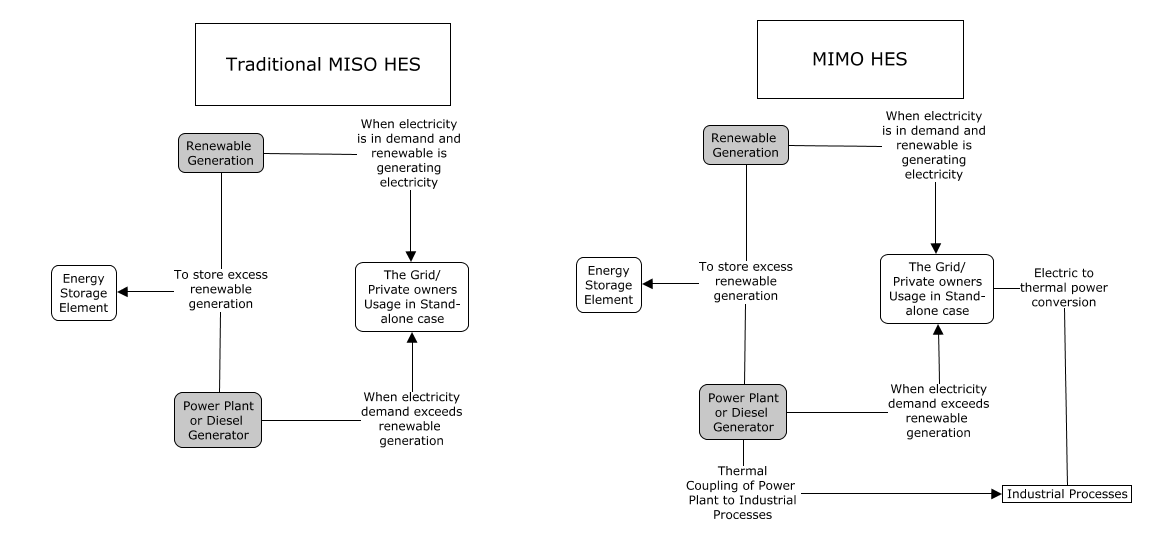
\includegraphics[width=\textwidth]{MISO_MIMO.png}
\caption{\small \sl This figure compares the MISO and MIMO configurations, demonstrating the differences between traditional hybrid energy systems that are focused on generating reliable electricity and non-traditional hybrid energy systems, which have the added objective of generating an additional product.  While many of the elements are the same, the MIMO system includes an Industrial Process  that is either thermally or electrically coupled.}
\end{figure*}

\section{Nuclear Renewable Hybrid Energy Systems}
Nuclear Renewable Hybrid Energy Systems (NRHES) are defined by Bragg-Sitton et al. (2014) as the "tighter coupling of nuclear and renewable energy sources in a manner that better optimizes energy use for the combined electricity, industrial manufacturing, and transportation sectors capable of apportioning thermal electrical energy to first meet the grid demand (with appropriate power conversion systems), then utilizing excess thermal and, in some cases, electrical energy to drive a process that results in an additional product \cite {Bragg-Sitton2014}".  The benefits to the participants of the NRHES that co-locate their facilities include minimizing system wide costs to the NRHES while increasing economic resilience by diversifying both the means of generating energy as well as the products produced. For example, if natural gas prices increase, the NRHES could rely less on the natural gas plant and put more focus on storage.  If short-term electricity prices are negative, the energy produced by the NRHES can be diverted to the industrial process.

The additional industrial products include, but are not limited to: synthetic fuel, titanium, desalinated water, hydrogen, aluminum, and heat pumps \cite{Bienvenue2015}. The NPP diverts the energy it generates between the grid and the industrial process to maximize profit. The system can allocate energy based on the market value of each of the multiple outputs produced. In the case of a NPP coupled with a desalination plant, for example, if the price of electricity is low, more thermal and/or electric energy can be diverted to generate more clean water at a higher profit \cite {Chen2016}. The costs of running a dynamic system, such as the case with a NRHES, include additional wear and tear, decreased thermal efficiency  due to variability, and increased complexity of operations  \cite{Garcia2013}. The total net costs of the system, such as meeting regulatory expectations , have yet to be determined.

\section{Ongoing Modeling Research}
There have been no physical demonstrations to date of NRHES. Therefore, research has largely focused on computational modeling to determine the feasibility and optimization of coupling elements \cite{Rabiti2015, Boardman2013, Shropshire2012}. Our literature review revealed that much of the work on NRHES is in the design and analysis stage \cite{Epiney2016, Boardman2013, Shropshire2012}. Research has focused on developing models that can dynamically simulate the contributions of variable energy sources, the constraints of fluctuating electricity demand, and thermal/electrical power demands for various industrial processes. The models focus on answering questions regarding minimizing the cost of electricity and ensuring profitability for each of the components comprising the NRHES. In order to move forward with development of any NRHES, such systems must demonstrate that they can be profitable and can reliably respond to fluctuating electricity production and demand \cite{Rabiti2015}.

An ongoing effort at \ac{inl}, \ac{anl}, and \ac{ornl} focuses on modeling a generic NRHES to optimize the size of the components as well as the overall functioning of the system. The generic nature of the plant means that regional variability in the renewable energy produced as well as the costs of the feedstocks for each of the systems is not taken into consideration. The generic model will test the economic viability of NRHES to determine if future development should be pursued. The industrial plant combines a nuclear power plant, a wind farm, a natural gas power plant, a battery, and a high temperature steam electrolysis hydrogen production facility. More component models will be developed in the future that can compare various industrial customers\cite{Harrison2016}. The chosen renewable source, a wind farm, models a highly stochastic system due to the unpredictable nature of wind generation \cite{Chen2016_wind}. The model optimizes the sizes of the nuclear power plant, the natural gas plant, and the battery. The model performs two optimizations, the first on the size of the components and the second optimizing the functioning of the system to minimize costs \cite{redfoot_rabiti_2018}. The objective is to choose the NRHES configuration that minimizes costs while meeting set emissions and grid reliability expectations.
\section{Computational Tools}
NRHES sit in an interesting location in computational modeling. There are many tools to model and optimize non-nuclear hybrid energy systems (HOMER, Hybrid2, SOLSIM, SOMES, ARES, RAPSIM, HOGA) \cite {Bernal-Agustin2009}. These programs generate mass flow and calculate electricity output and the possible output of another product, such as hydrogen. Modelica and Excel, while neither specifically HES nor NRHES tools, have been used to model both nuclear and non-nuclear hybrid energy systems \cite{Shropshire2012, Chen2016, Binder2014, Garcia2015, Epiney2016}. HES tools are typically developed for microgrid standalone systems. The main challenges to applying HES systems to a NRHES are the scale of the system being modeled and fluctuating grid demand.
% Need to add some more review of why HOMER cannot be used to model a NRHESSince microgrid systems are typically used for off grid modeling, they do not include
\section{NRHES Models}
Selecting a tool to model a NRHES requires understanding what characteristics a model must possess in order to provide accurate information. For example, as discussed below, it is important for a NRHES model to incorporate the dynamic nature of the system in order to include losses from the fluctuations in the system. Understanding the differences among the underlying mathematical models as well as the software functionality is essential in determining whether and how a nuclear fuel cycle simulator (NFCS) will be useful to NRHES modeling.
As mentioned above, the model currently under development by \ac{ornl}, \ac{anl}, and \ac{inl} has reviewed the essential characteristics for a computational model of NRHES. Rabiti et al. (2015) discusses the important elements of a NRHES computational model in detail, describing the basic requirements of the software as a "computational representation of the thermal, mechanical, chemical, and electrical processes in the systems as process units, reactors, manufacturing plants, and energy delivery (to the appropriate point of interface with the market transaction, such as an electricity bus, or a product depot or distribution terminal where a commodity price is established)"\cite{Rabiti2015}. The model in development by the national laboratories combines \ac{raven} for the stochastic and statistical aspects of the system, such as generating synthetic wind data and optimizing the systems with Modelica for modeling the various components in the NRHES.
\subsection{Modelica}
Modelica is a widely used open source language for modeling large and complex systems composed of smaller component models. It is particularly optimized for modeling dynamic systems. Modelica has powerful libraries, such as Thermopower, that include the thermohydraulic modeling tools required for modeling mass flows in energy systems \cite{Binder2014}. The language is well-maintained, giving it the added benefits of having up-to-date documentation and a community that can provide support. Typically Modelica is run on the Dymola developer environment, a private tool developed by the creator of Modelica, Dr. Hilding Elmquist. Another option for running the Modelica language is the open source OpenModelica environment.

A Modelica HES model developed in Binder et. al. (2014) includes a nuclear reactor, two steam cycles, a chemical plant, and an electrical component \cite{Binder2014}. The products of this Modelica NRHES model are synthetic fuel and electricity. The model includes the ramp up stage when the reactor initially starts or is increasing from a lower load. The steam generator connected to the NPP determines which of its turbines to use depending on electricity demand, the 60\% turbine, the 30\% turbine, or the 15\% turbine, which can be used in unison. A pressure relief valve releases excess energy unused by the turbines. The wind generation is modeled using the Western Wind dataset from the \ac{nrel} for an unspecified region in Idaho. Each component in the model was tested individually before being combined. Using the individual component models, verifications were made for the system as a whole. The startup transient state of the model took much greater computation time due to the complex interrelations of the components. Generally, running a model of a NRHES in Modelica requires a control algorithm, a differential equation that controls how the dynamic system allocates heat. The profitability control algorithm can be adjusted to incorporate varying parameters such as the price of electricity or the cost of natural gas. The study concluded that Modelica, due to its ability to evaluate control algorithms, is an effective tool for dynamically modeling a HES. As a tool that is optimized for large dynamic systems, Modelica has been used more than any other tool to model NRHES at this point.

\subsubsection{RAVEN}
The RAVEN tool was initially built for probabilistic risk assessment. RAVEN, as a probabilistic tool, can do parametric and stochastic analyses of systems\cite{RabitiRAVEN}. For the NRHES, RAVEN is used to run different wind energy generation paths in order to generate a statistically fair representation of how renewables, in this case wind power, would likely function over any given hour. RAVEN can be used to generate the most generic seasonal wind generation over a week. A typical week can be extrapolated to represent a given season. The process can be repeated over the different seasons, which can be extrapolated to represent a year. Using synthetic generated data instead of historic data avoids the critique that the model only represents past behavior and is thus inapplicable to future trends \cite{redfoot_epiney_2016}. RAVEN can also be used to determine high-risk time series samples to ensure that high risk scenarios are accounted for in the study. RAVEN can also do probabilistic assessments such as loss of load probability and sensitivity to uncertainty analysis.

Any future modeling efforts for a NRHES would benefit from complimenting the ongoing modeling effort. Currently, all of the physics models for the NRHES are built in Modelica. To benefit from the work already done, any additional software would need to be able to easily communicate with the Modelica modeling language.  The model would benefit from a tool that would communicate with other chemical and utility standard physics modeling tools. Future work would benefit from coupling with other physics modeling tools, allowing groups to take advantage of the existing infrastructure while using their physics model of choice.

\subsection{Distinct Capabilities}
There are certain characteristics of a physical NRHES which a computational model would need to have to be a reasonable assessment of the system as a whole. Table I below demonstrates the functions which are most commonly incorporated in a model. I discuss dynamic modeling explicitly as it is the capability highly valued in a NRHES that is not nearly as important in a NFCS. The below discussion details the extensive work that has been done determining why a dynamic system is important to a NRHES.

In Garcia et. al. (2013) and Du et. al. (2014), a dynamic approach to modeling hybrid energy systems (HES) is applied in order to appropriately address the impacts of flexible operation of the system due to variable renewable generation \cite{Garcia2013, Du2014}. In Du et. al. (2014), two optimization problems are addressed: the first minimizes variability in the HES through optimizing components of the HES system, and the second imposes operating and capital costs on the design variables. Garcia et. al. (2013) has a two-part series. The first applies and analyzes performance of a dynamic approach to modeling some of the physical components of a traditional and an advanced (produces goods besides electricity) HES. The second paper focuses on economic effects using a dynamic approach, as opposed to time series or statistical analysis. Overall, both parts of the series focus on how a dynamic approach better models the high level of variability of a HES for output generation and profitability maximization \cite{Garcia2013}. The costs of operating in a flexible manner, dynamically allocating resources between multiple coupled systems, are substantial enough to require a simulation that precisely models the variability of the system \cite{Garcia2013, Shropshire2011, Locatelli2015}. The dynamic modeling at this point focuses on the dynamic transfer of energy to different sources, and how this impacts the economics and grid reliability. The physical impacts of the grid system have not yet been included in the model \cite{Harrison2016}.  The dynamic allocation of the heat and electricity depending on the renewable generation and the grid demand is an essential characteristic of a NRHES.  Including factors such as how quickly the NRHES will be able to switch between providing energy to the industrial facility and the grid will impact determining the economic and physical values of the model.

\section{Small Modular Reactors}
For completeness, the use of \ac{smrs} both as tools for load following and as sources of process heat must be addressed. SMRs are generally defined as nuclear reactors under 300 MWe. SMR designs, such as the one in development by NuScale, combine multiple small reactor modules. Multiple SMRs in combination are a promising possibility for NRHES.  With multiple reactors, individual modules can be assigned to meet the industrial process energy demand, with others solely used for electricity generation. Furthermore, as electricity demand grows, additional modules can be added to the industrial park. Multiple SMRs have a clear means of load following, simply by shutting down those reactors whose energy output is not required due to seasonal shifts and other demand factors. The modularity of the SMRs allows greater flexibility in the design of the industrial park.  Locatelli (2015) discusses the technical and economic feasibility of load following using multiple SMRs, applying the excess energy toward generating algae-biofuel and desalinated water \cite{Locatelli2015}. He discusses the benefits as well as drawbacks of an NRHES that includes a thermal desalination process. A desalination plant has the benefits of switching between a latent and producing state and generating a product that is readily stored. The main drawback is poor water quality and output level when the desalination unit restarts.

The NuScale reactor, with proposed construction starting in 2025 at Idaho National Laboratory, has motivated research into different methods of fluctuating the amount of electricity sent to the grid \cite{Ingersoll2014, Ingersoll2015, Ingersoll2016, Ingersoll2014_1}. The NuScale reactor design, as can be seen in the figure below, combines twelve small pressurized water reactors into one large pool of water.  Each of the reactors is rated at 50 MWe,generating a combine 600 MWe. The NuScale reactor has been evaluated to thermally couple with oil refining processes, multiple desalination techniques, as well as hydrogen production \cite{Ingersoll2014}. Besides from thermally coupling and rerouting the energy from electricity generation to process heat applications, the NuScale reactors have furthermore been evaluated for loosely coupling with the Horse Butte Wind Farm in nearby Idaho Falls \cite{Ingersoll2015}.  The NuScale plant has multiple approaches to meeting the fluctuating electricity demanded by the grid, which NuScale designates as NuFollow \cite{Ingersoll2015}.  The NuScale plant can take down one or more of the low power reactors, changing the power output of one or more modules for shorter changes in the grid demand due to changes in wind output, and sending the heat generated by the reactor straight to the condenser bypassing the power generating turbine cycle.
\begin{figure*}[h!]
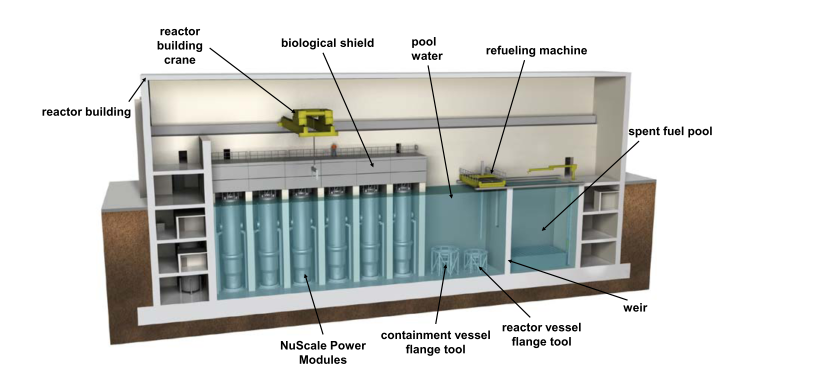
\includegraphics[width=\textwidth]{NuScale_cutaway.PNG}
\caption{\small \sl This figure displays the design of half of the NuScale module. Six of the reactor modules can be seen in the cooling pool along with the crane which inserts and removes the modules.}
\end{figure*}
\subsection{Other Research on NRHES Models}
Many more studies on HES and NRHES incorporate economic and technical modeling, but the essential characteristics of ability to model a dynamic and stochastic system have been covered. For completeness of the state of the art research on NRHES, some of the other relevant studies include:
\begin{itemize}
\item Shropshire et. al. (2012) does not focus on HES, but discusses how different models of flexible and small modular reactors could integrate into the European energy market with growing renewable generation, thus fulfilling the growing need for flexibility and load following in other electricity suppliers \cite{Shropshire2012}.
\item Shropshire et. al. (2011) develops target cost estimates for reactors given certain economic environments based on competing technology energy costs \cite{Shropshire2011}.
\item NEA-OECD (2011), Nuclear Energy Agency Organisation for Economic Co-operation and Development, presents an overview of the capability of implemented newer and older nuclear power plants to load follow \cite{Nuclear2011}.
\item Baker (2016) analyzes the \ac{lcoe} as the \ac{fom} and the role of battery storage to evaluate different NRHES scenarios \cite{Baker2016}
\item Kazimi et al. (2009) produces a preliminary dynamic analysis of two NRHES systems that have high levels of renewable energy generation and multiple outputs from the system. The study concludes that NRHES could lead to optimized energy use, reduced carbon, favorable economic performance, and flexible operation time \cite{Kazimi}.
\item Forsberg et. al. (2009) discusses using nuclear power to create more liquid transportation fuels from biomass and fossil fuel sources \cite{Forsberg2009}.
\item There have also been two regional modeling studies done on Texas and Arizona focused on including regional characteristics to determine the renewable used and the industrial process.
\end{itemize}
Table I displays the characteristics routinely described as necessary to model a NRHES along with their citations.

\begin{table}[h!]
\centering
\caption{References for Each NRHES Characteristic}
\begin{tabular}{ ||c | c|| }
 \hline
 NRHES Characteristic & Paper \\ [0.5ex]
 \hline \hline
 Dynamic & \cite{Garcia2013, Du2014, Kazimi, Garcia2016}\\
 \hline
 Sensitivity Analysis & \cite{Shropshire2011, Rehman2010, Adaramola2014, Chen2016}\\
 \hline
 Optimization of components & \cite{Chen2016,Ozcan2016, Forsberg2009,Garcia2015,Aumeier2011}\\
 \hline
 Stochastic Model of Renewables & \cite{Rabiti2015, Garcia2016,Locatelli2015}\\
 \hline
 Grid Demand model & \cite{Forsberg2013, Garcia2016,Garcia2013,Ruth2014,Chen2016}\\
 \hline
  Economic FOMs & \cite{Garcia2016,Chen2016,Rabiti2015,Epiney2016,Bragg-Sitton2014}\\
 \hline
\end{tabular}
\label{table:1}
\end{table}

The table displays the characteristics that arise as a pattern in many of the documents.  The six characteristics included in the table are those likely necessary for a NRHES model.  Each of the characteristics has been included in previous studies, and thus has some already proposed approaches.  The characteristics can be studied in greater detail in order to determine if they satisfactorily model the system.

\chapter{Figures of Merit}
To determine the performance of an electrically coupled versus a thermally coupled NRHES, clear performance criteria must be established.  While economic figures of merit must be evaluated for a NRHES, other benefits of the system such as grid reliability and safety of the system should also be considered. This section of the thesis details the current efforts at establishing a figure of merit to analyze a NRHES and suggests a levelized costs of feedstock approach found throughout industrial ecosystem literature.
\section{Economic Figures of Merit}


\subsection{Levelized Cost of Electricity}
The levelized cost of electricity (LCOE) is the typical FOM for comparing the profitability of different generating sources, such as nuclear, fossil fuels, and renewables. The LCOE is mathematically defined as the costs of a power-generation source divided by the total energy output, with units of \$/unit of energy. The LCOE is easiest to think about as the lowest average amount of money a project can sell the electricity generated for over its lifetime in order to break even, or for the \ac{npv} (discussed below) to equal zero. The LCOE is a ubiquitous metric used for evaluating energy generation sources, but it is not always calculated the same way.  The two equations below illustrate very different means of calculating a figure bearing the same name.  While a lack of clarity about what is meant by LCOE can be mitigated by defining the means of calculating the value, this practice is often overlooked.

\begin{figure*}[h!]
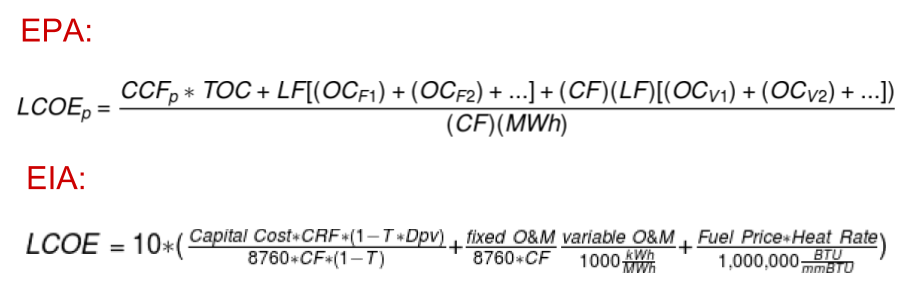
\includegraphics[width=\textwidth]{LCOE_EIA_EPA.png}
\caption{\small \sl These equations display two different definitions of Levelized Cost of Electricity from two government organizations demonstrating the issues surrounding even understanding the meaning of current economic figures of merit applied to electricity.  Equations come from \cite{Eia2017} and }
\end{figure*}


Ted Baker, in Analysis of Nuclear Hybrid Energy Systems with Battery Storage Using Levelized Cost of Electricity, evaluated the effectiveness of the \ac{lcoe} for a hybrid system \cite{Baker2016}. His analysis found the LCOE was incapable of fully capturing the benefits of energy storage associated with a NRHES and did not including all revenue streams.  Baker defines the utilization as energy used divided by the total possible generation. In order to normalize the LCOE, the calculated LCOE shown in equation 1 below is multiplied by the total energy actually used for each source.  As Baker describes, to normalize the LCOEs "the sum of all specific LCOEs is then divided by the sum of the demand data. This weights each source by its contribution to coverage (pg. 20)."  The revenue rate of the secondary product in \$/MWh is subtracted from the total LCOE in order to find the net LCOE.  Baker concludes that the LCOE is ineffective for the revenue stream of a secondary product and includes errors for variable generation and battery storage. Baker recommends exploring more advanced LCOE and \ac{lcs} calculations. The LCS focuses on comparing the costs between various energy storage sources optimizing for different use cases \cite{Tyskiewiczd}.

\begin{figure*}[h!]
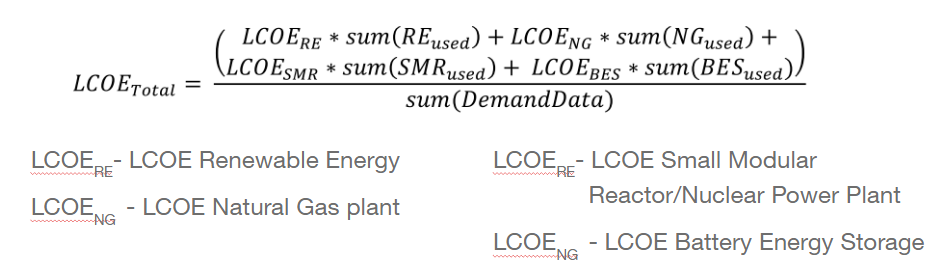
\includegraphics[width=\textwidth]{Hybrid_LCOE.PNG}
\caption{\small \sl This equation displays the combined Hybrid Energy System Levelized Cost of Electricity comprised off the LCOEs of each of the components multiplied by which portion of the electric market was actually met by that generation source \cite{Baker2016} }
\end{figure*}


\subsection{Levelized Avoided Cost of Electricity}
The \ac{lace} evaluates the value of a new generation project by assessing what costs to the grid the new generation would replace. The LACE accounts for the variability across different regions by focusing on the costs of generating electricity by the sources the new generation project would replace, be it a coal plant, a natural gas plant, a nuclear plant, etc.  The EIA suggests using the LACE in combination with the LCOE when determining the best generation source for a given region \cite{Eia2017}. The supplement to EIA, 2017 specifies how they calculated the LACE.


\begin{figure*}[h!]
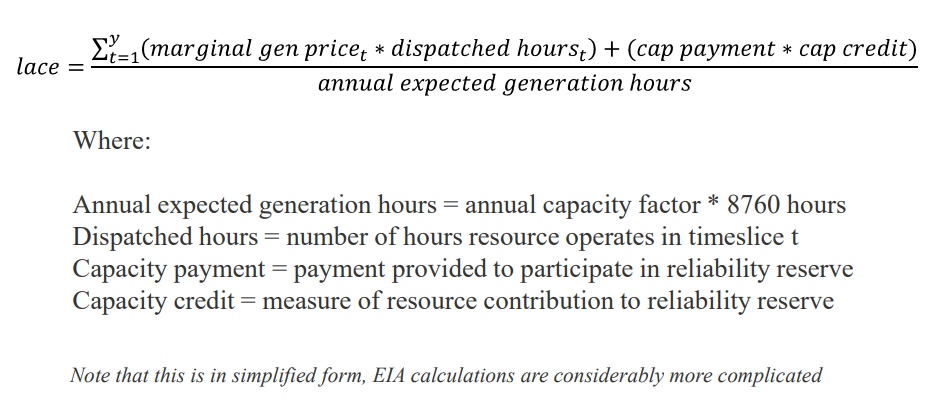
\includegraphics[width=\textwidth]{LACE.PNG}
\caption{\small \sl The calculation provides a simple conceptual representation of how the LACE is determined. Though, there is a note demonstrating that this is not the actual calculation used when the \ac{eia} finds the LACE. \cite{Namovicz2013} }
\end{figure*}



\subsection{Net Present Value}
Net Present Value as defined by Harvard Business Review, is "the present value of the cash flows at the required rate of return of your project compared to your initial investment \cite{Gallo}." The basic \ac{npv} equation is:
\begin{equation*}
NPV=\sum_{t=1}^T\frac{Cash\hspace{.2 cm}Flow_t}{(1+i)^t}-Initial\hspace{.2 cm}Cash\hspace{.2 cm}Investment
\end{equation*}

The NPV analyzes if the money invested in a project will make more profit over its lifetime than simply leaving the money in the bank, or a seperate investment.  NPV is a metric that allows comparisons of the likely profits of NRHES with different industrial processes.  The NPV determines the lifetime LCOE of a project by finding the internal rate of return.  The \ac{irr} is the interest rate at which the NPV of all the cash flows equal zero.  The IRR is the interest rate that either the money spent on the NRHES would earn if it is kept in the bank, or the profit over the lifetime NRHES would earn.  In order to appropriately value all of the characteristics of an NRHES, the figure would need to include a grid reliability metric and a value for non-emitting energy. These values could come from suggested carbon taxes, likely increases in healthcare expenditures due to emissions, as well as the costs of blackouts.

\section{Grid Reliability}
A hybrid energy system in general has not only a goal of profitability, but to ensure a reliable source of energy, especially from a system that includes fluctuating sources of energy. The system would, therefore, benefit from an evaluation of the reliability of the energy generated as well as an economic evaluation.
\subsubsection{Loss of Load Probability}

The \ac{lolp} measures the probability the load on a system will exceed the electricity available. Generally, the LOLP is expressed as the estimated number of days over a time duration, often 10 years or the life of the system, that the system will be unable to meet the demand. The LOLP was originally introduced in 1947 by Giuseppe Calabrese and has since become a standard grid reliability metric \cite{calabrese1947generating}. The LOLP can be mathematically shown, as described in Hattab et. al. (2015), as \cite{Hattab2015}:
\begin{equation*}
LOLP =\sum_{j} P_jt_j\,.
\end{equation*}

Where P(j)*t(j) is the contribution that a particular outage of some magnitude O(j) has on the overall risk of a load greater than the reserve. t(j) is the number of days that an outage of some magnitude O(j) would cause a loss of load in the system\cite{Hattab2015}.



\subsubsection{Industry Standards for Grid Reliability}
For completeness, I will quickly discuss the two figures of merit used by electric power utilities to measure grid reliability.  The two metrics are the \ac{saidi} and the \ac{saifi}. While these figures of merit are not currently applicable to NRHES, as real data is required, they will be used in the future.  These figures of merit can also be applied to potential simulations where a certain population is assumed to be served by the NRHES.

\begin{equation*}
SAIFI =\frac{total\hspace{.15 cm} number\hspace{.15 cm} of\hspace{.15 cm} customer\hspace{.15 cm} interruptions}{total\hspace{.15 cm} number\hspace{.15 cm} of\hspace{.15 cm} customers\hspace{.15 cm} served}
\end{equation*}

\begin{equation*}
SAIDI = \frac{sum \hspace{.15 cm} of \hspace{.15 cm}all \hspace{.15 cm}customer\hspace{.15 cm}interruption \hspace{.15 cm} durations}{total\hspace{.15 cm}number\hspace{.15 cm}of\hspace{.15 cm}customers\hspace{.15 cm}served}
\end{equation*}

NRHES, since they would be operating in a fluctuating way, may be considered dispatchable energy sources. As defined by NERC standards, dispatchable energy must be able to get to full capacity on the grid in ten minutes.  The rapid time requirement has made it impossible in the past for nuclear to be considered dispatchable.  With a NRHES, especially one that is electrically coupled, the system could be able to allocate electricity quickly. With nuclear, renewables, and likely a battery or natural gas plant all contributing, the considerable backup allows for a fairly large range of load to be met be a NRHES potentially. For a NRHES, two LOLPs must be generated; one for meeting the electricity demand from the grid and one for meeting the energy needs of the industrial process.  If the industrial process intends to fluctuate its output along with the energy generated from renewable and the grid demand, the losses from the industrial process will need to be taken into consideration for grid reliability. In order to fairly evaluate the benefits of an NRHES, metrics describing the system need to include a grid reliability component.  The technical benefit of coupling nuclear and renewables is reliable low emissions energy. Without considering the reliable aspect, a major value is left unconsidered.

Eventually, the goal is to determine a figure of merit that is able to incorporate grid reliability and profitability metrics.  The profitability metrics will include the materials replacement rates for different reactor types, industrial processes, and heat transport mechanisms. Future work will include emissions in the FOM. Since at this point, standard figures of merit have not been established for NRHES, this research will work to determine some combination to evaluate the systems.

\section{Levelized Cost of Feedstocks}
There is a whole academic focus on industrial ecosystems.  The most famous of which is the Kalundborg industrial park in Denmark. The Kalundborg system is comprised of  Both an exergy analysis as well economic and environmental assessments have been done on the Kalundborg system \cite{Valero2012,Jacobsen}.  The general comparison done with these analyses is between the costs and impacts associated with the combined system as opposed to if each of the components were separated.
%an   as well as other industrial ecosystem background and the general approach of comparing the coupled system to an uncoupled system in terms of costs.  Discuss the need to put a monetary value on the ability to fluctuate.

\begin{figure*}
\centering
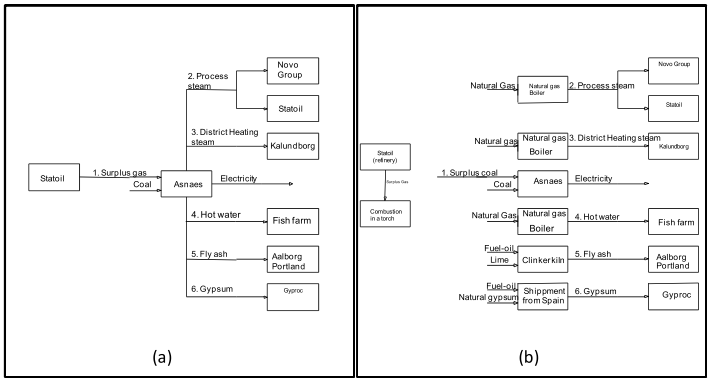
\includegraphics[width=.7\textwidth]{kalundborg_cases.PNG}
\caption{\small \sl This figure displays the two cases evaluated in Valero et. al. Figure a shows the industrial ecosystem in the current coupled form. Figure b shows the second case where there is no coupling.}
\end{figure*}

%Here ends what I will send for a review to my committee.

\chapter{Applying Risk Assessment Techniques to NRHES}
Identifying likely failures is an important aspect of safe and secure operation of any large infrastructure. For a NRHES, a large piece of infrastructure that has as of yet to be built, a design that addresses likely failures ensures long term safe, reliable, and profitable operation. This chapter will evaluate the economic, grid reliability, and physical risks of failures in the coupling of a nuclear power plant to an industrial process which functions in a dynamic fashion. Three preliminary hazard analyses will initially be applied to the safety, ability to fluctuate, profitability of the system in order to do a cursory qualitative model of what concerns need to be taken into consideration. A fuzzy \ac{ahp} will then be applied to various industrial processes coupled with an NRHES. The focus of this section is to develop a means of comparing various NRHES industrial processes to determine which industrial process will be used in the exergy analysis.
\section{Risk Assessment Background}
Risk assessment is a means of analyzing complex systems for hazards. Often the risk assessment tools; such as probabilistic risk assessment, fault tree analysis, and failure mode and effects analysis; model many variables in large systems and attempt to contain them into an easy to understand table or number for comparison. Since there has yet to be a physical model of a NRHES built, now is the appropriate time to assess risks in order to incorporate mitigating measures in the design basis. Incorporating risk management in the design of a facility minimizes the costs and dangers associated with the system in the long run.
%When determining an appropriate electricity generation source for a given region it is important to incorporate variables such as economic viability, emissions, flexibility, and reliability. A NRHES is even more difficult to quantify as it supplies both electricity to the grid as well as a secondary product. The goal is to have a more economically robust system that emits less and is both more reliable and more flexible than any electricity generation source currently available.

\section{Preliminary Hazards Analysis}
As was done in Falcone et. al. in establishing a new approach to risk assessment of cogeneration systems, this risk assessment will begin with a \ac{pha} \cite{Falcone}. The main purpose for a PHA is, as the name suggests, identify hazards and possible implications of the design of a particular system or product.  A PHA is appropriate for the current state of development for a NRHES due to it still being in the design stage. The goal of this PHA will be to reduce or eliminate potential economic, reliability, and physical safety hazards. Performing a PHA at this early point in the lifecycle of a NRHES will hopefully reduce the resources spent on engineering design and potential construction errors. This analysis is not exhaustive but will address some of the more obvious concerns. The PHA will need to be added upon as research continues and hazards are determined.
	In order to perform a PHA requires classifying the hazard level and frequency associated with each event. The hazard classes for this PHA range from Negligible to Catastrophic. A Class I hazard has negligible negative outcomes, a Class II hazard has marginal effects, a Class III hazard has critical impacts, and a Class IV hazard has catastrophic impacts\cite{ostrom2012risk}.  The frequency of occurrence, since this system has yet to have a physical demonstration, will be qualitative as the values cannot be verified at this point.

\begin{landscape}
%\subsubsection{Economic PHA}
\begin{table}[h!]
\centering
\caption{Economic Preliminary Hazard Analysis}
\label{my-label}
\begin{tabular}{|l|l|l|l|l|l|}
\hline
\textbf{\begin{tabular}[c]{@{}l@{}}Potential \\ Failure\end{tabular}} & \textbf{\begin{tabular}[c]{@{}l@{}}Event Causing\\ Hazardous\\ Condition\end{tabular}} & \textbf{\begin{tabular}[c]{@{}l@{}}Hazardous\\ Condition\end{tabular}}  & \textbf{Hazard Class} & \textbf{\begin{tabular}[c]{@{}l@{}}Preventative \\ Measure\end{tabular}} & \textbf{\begin{tabular}[c]{@{}l@{}}Qualitative\\ Likelihood\end{tabular}} \\
\hline
\begin{tabular}[c]{@{}l@{}}Industrial process\\ is not profitable \end{tabular}      & \begin{tabular}[c]{@{}l@{}}If the industrial\\ process has to be\\ ready to take load\\ from the grid, it \\ will likely be running\\ below capacity and \\ may not be profitable\end{tabular}      & \begin{tabular}[c]{@{}l@{}}Industrial \\ process loosing\\ money\end{tabular} & \begin{tabular}[c]{@{}l@{}}Class III,\\ the benefit of\\ the NRHES \\ would be lost\\ without a means\\ of having the \\ industrial process\\ prepared to take \\ heat. \end{tabular}    & \begin{tabular}[c]{@{}l@{}}Contracts \\ ensuring\\ a certain profit\\ for the industrial\\ process to be \\ prepared to \\ take heat from\\ the Nuclear\\ Power Plant\end{tabular} & Likely \\
\hline
\begin{tabular}[c]{@{}l@{}}Nuclear regulations \\ could apply to the\\ whole system, \\ increasing the costs\\ of the system\end{tabular} & \begin{tabular}[c]{@{}l@{}}Since the \\ components will \\ be co-located \& \\ coupled, the NRC \\ may have\\ jurisdiction \\ over the whole system\end{tabular}  & \begin{tabular}[c]{@{}l@{}}Additional \\ regulations \\ on the industrial \\ process could \\ result in greater\\ costs\end{tabular} & \begin{tabular}[c]{@{}l@{}}Class III: without an \\ industrial process\\ the whole NRHES \\ would be undermined.\end{tabular} & \begin{tabular}[c]{@{}l@{}}Determine regulatory \\ oversight before \\ beginning \\ construction\end{tabular} & \begin{tabular}[c]{@{}l@{}}Fairly Likely\\ as the other\\ components\\ would be\\ within the\\ required \\ boundary \\ around the NPP\end{tabular} \\
\hline
Feedstock costs rising & \begin{tabular}[c]{@{}l@{}}Any of the feedstocks\\  could rise in price for \\ any number of reasons. \\ Rise in price during \\ the operation of the \\ system could result in \\ the product prices no \\ longer being\\ competitive\end{tabular} & \begin{tabular}[c]{@{}l@{}}Feedstocks rising in \\ price during the \\ operation of the system \\ could\\ result in the \\ product prices no \\ longer being \\ competitive\end{tabular} & \begin{tabular}[c]{@{}l@{}}Class I: shifts \\ already occur in\\ feed stock prices and\\ are systems adjust.\end{tabular}  & \begin{tabular}[c]{@{}l@{}}Include long term \\ projections for the \\ feedstock costs of \\ the various \\ components in the \\ design phase of the \\ NRHES\end{tabular}                      & \begin{tabular}[c]{@{}l@{}}Likely there \\ will be \\ fluctuations.\\ Depends on the \\ feedstock\end{tabular}\\
\hline
Product value decreasing & \begin{tabular}[c]{@{}l@{}}There could be a \\ change in \\ conditions or a \\ new technology \\ that makes the \\ industrial process \\ product value \\ decrease\end{tabular} & \begin{tabular}[c]{@{}l@{}}For each of the products,\\ the reason would be \\ different. Desal: a \\ drought could end\\ Syn fuel: oil prices \\ could decrease\\ Hydrogen: Less \\ energy\\ intensive \\ process could be \\ invented\end{tabular} & \begin{tabular}[c]{@{}l@{}}Class II: the industrial \\ process would need\\ to be further subsidized\\ by other components \\ to continue to run\end{tabular}& \begin{tabular}[c]{@{}l@{}}Do long term \\ economic \\ analysis of the \\ industrial \\ process. Pick \\ a product \\ or location where\\ the product will \\ clearly be in demand\end{tabular} & \begin{tabular}[c]{@{}l@{}}Possible: The \\ product value \\ will likely \\ fluctuate over \\ the length of \\ the\\ project\end{tabular}          \\ \hline
\end{tabular}
\end{table}                                           \end{landscape}

\begin{landscape}
%\subsection{Grid Reliability PHA}
\begin{table}[h!]
\centering
\caption{Grid Reliability Preliminary Hazard Analysis}
\label{my-label}
\begin{tabular}{|l|l|l|l|l|l|}
\hline
\textbf{\begin{tabular}[c]{@{}l@{}}Potential \\ Failure\end{tabular}} & \textbf{\begin{tabular}[c]{@{}l@{}}Event Causing\\ Hazardous\\ Condition\end{tabular}} & \textbf{\begin{tabular}[c]{@{}l@{}}Hazardous\\ Condition\end{tabular}} & \textbf{Hazard Class} & \textbf{\begin{tabular}[c]{@{}l@{}}Preventative \\ Measure\end{tabular}}  & \textbf{\begin{tabular}[c]{@{}l@{}}Qualitative\\ Likelihood\end{tabular}} \\
\hline
\begin{tabular}[c]{@{}l@{}}Nuclear Power \\ Plant Outage\end{tabular}  & \begin{tabular}[c]{@{}l@{}}The NPP needs \\ to be refueled\end{tabular} & \begin{tabular}[c]{@{}l@{}}NPP down for \\ refueling\end{tabular} & \begin{tabular}[c]{@{}l@{}}Class I: This will \\ be a routine issue. \\ The industrial \\ process will need \\ to stop during the \\ outage and the \\ grid will need to \\ get electricity \\ from peaker\\ plants\end{tabular} & \begin{tabular}[c]{@{}l@{}}Plan ahead with the \\ industrial process \\ so that it can either \\ get\\ electricity from\\ the grid or be \\ paid to close for \\ the outage.\end{tabular}                                     & \begin{tabular}[c]{@{}l@{}}Certain: an \\ NPP needs to \\ be refueled\end{tabular} \\
\hline
\begin{tabular}[c]{@{}l@{}}System not able \\ to quickly shift\\  heat from \\ industrial process \\ to\\ electricity \\ generation\end{tabular} & \begin{tabular}[c]{@{}l@{}}The NPP heat \\ transport system \\ taking a while to \\ shift.\end{tabular} & \begin{tabular}[c]{@{}l@{}}The NRHES is \\ briefly unable \\ to meet \\ the grid demand\end{tabular} & \begin{tabular}[c]{@{}l@{}}Class II: There \\ would be some \\ money loss as \\ some other \\ electricity \\ generation system \\ would supply the \\ demanded energy \\ during the transition \\ period\end{tabular}            & \begin{tabular}[c]{@{}l@{}}Include the time it \\ takes to allocate \\ heat in models of \\ the NRHES to \\ determine how \\ much of a limiting \\ factor it is likely to be.\\ Include a battery in\\ the NRHES\end{tabular} & Likely \\                       \hline
\end{tabular}
\end{table}
\end{landscape}



\begin{landscape}
%\subsection{Physical PHA}
\begin{table}[h!]
\centering
\caption{Physical Preliminary Hazards Analysis}
\label{my-label}
\begin{tabular}{|l|l|l|l|l|l|}
\hline
\textbf{\begin{tabular}[c]{@{}l@{}}Potential \\ Failure\end{tabular}}                        & \textbf{\begin{tabular}[c]{@{}l@{}}Event Causing\\ Hazardous\\ Condition\end{tabular}} & \textbf{\begin{tabular}[c]{@{}l@{}}Hazardous\\ Condition\end{tabular}} & \textbf{Hazard Class} & \textbf{\begin{tabular}[c]{@{}l@{}}Preventative \\ Measure\end{tabular}} & \textbf{\begin{tabular}[c]{@{}l@{}}Qualitative\\ Likelihood\end{tabular}}                 \\
\hline
\begin{tabular}[c]{@{}l@{}}Materials failure \\ in the heat \\ transport system\end{tabular} & \begin{tabular}[c]{@{}l@{}}NRHES are very \\ dynamic systems. \\ There will likely \\ be greater materials \\ wear due to the \\ dynamisticity of \\ the system\end{tabular} & \begin{tabular}[c]{@{}l@{}}Heat transport \\ pipe forms a leak\end{tabular}            & \begin{tabular}[c]{@{}l@{}}Class III:There \\ would be a loss \\ of\\ money due \\ to the shutdown \\ of the system\end{tabular}                                                                                                          & \begin{tabular}[c]{@{}l@{}}Reliable maintenance \\ \& appropriate choice \\ of heat transport \\ system\\ materials\end{tabular} & Possible                                                                                  \\
\hline
Release of Radionuclides                                                                     & \begin{tabular}[c]{@{}l@{}}A lot of things \\ would need to \\ go awry\end{tabular}                                                                                          & \begin{tabular}[c]{@{}l@{}}A large release \\ of airborne\\ radionuclides\end{tabular} & \begin{tabular}[c]{@{}l@{}}Class IV: A \\ radiation release \\ that could \\ potentially impact \\ human health \\ would have\\ massive negative \\ impacts for the \\ nuclear industry \& \\ would shut down \\ the\\ NRHES\end{tabular} & \begin{tabular}[c]{@{}l@{}}Passive safety \\ systems, excellent \\ safety culture, \\ good reactor design\end{tabular}           & \begin{tabular}[c]{@{}l@{}}Unlikely: Based \\ on history of \\ NPP operation\end{tabular} \\
\hline
\end{tabular}
\end{table}
\end{landscape}


\section{Analytic Hierarchy Process}
The fuzzy AHP below compares NRHESs that include thermal coupling to three types of industrial processes: desalination, synthetic fuel production, and hydrogen production.  The paper will evaluate the profitability, flexibility, and safety characteristics in the coupling of a nuclear power plant to each of the given industrial processes. While AHP has been applied to energy systems in the literature, the application to NRHES is novel. An AHP approach provides important information into design considerations and quantitatively approaches which alternative is likely to be strongest given the criteria chosen. As NRHES are currently in the research and development stage, AHP is a beneficial tool to develop for future decision making for NRHES.

An AHP uses pairwise comparisons of various potential options depending on a set of predetermined characteristics. Originally developed in the 1970s by Thomas L. Saaty, AHP has been applied to everything from determining the appropriate bridge construction \cite{Pan2008}, to the appropriate energy make-up of Turkey\cite{Kahraman2010} \cite{Saaty1987}. AHP is a multicriteria decision-making tool. There is a wealth of research applying multicriteria decision-making tools to energy planning. Pohekar et al. reviewed more than 90 published papers on multi-criteria decision making and energy planning \cite{Pohekar2004}. Pohekar et al. found AHP to be the most popular multicriteria decision-making technique used in energy planning. The reasons for the prevalence of AHP in energy planning, Pohekar et al. suggests, is due to its ability to:
\begin{quote}
	convert a complex problem into a simple hierarchy, flexibility, intuitive appeal, its ability to mix qualitative as well as quantitative criteria in the same decision framework and use of computational aids leading to successful decisions in many domains.
 \end{quote}
Some of the previous applications of AHP to energy systems noted in Pohekar et al. include Akash et al.  1999; and Ramanathan et al. 1995. Akash et al. uses AHP to analyze the selection of power plants in Jordan \cite{Akash1999}.  Ramanathan et al. applies AHP at a household level in India to determine which energy resources work best for various tasks in the home such as heating, water pumping, lighting, and household appliances \cite{Ramanathan1995}.

The general process for applying AHP involves initially determining a set of alternatives and a set of criteria on which to compare the alternatives. To hierarchy comes from the objective being structured above the criteria, which is then structured above the alternatives, as can be seen in figure 3.1 below. To find the relative value of one of the alternatives over the other, the AHP approach develops a series of pairwise comparisons creating a ratio scale.  Generally AHP is done on a scale of one to nine. After creating the ratio scale, the AHP approach applies an eigenvalue method to include the relative weights of each of the criteria to each of  the elements. Finally, the relative weights are combined with the ratios forming one measurement to compare the various elements.

\begin{figure}[h!]
  \centering
  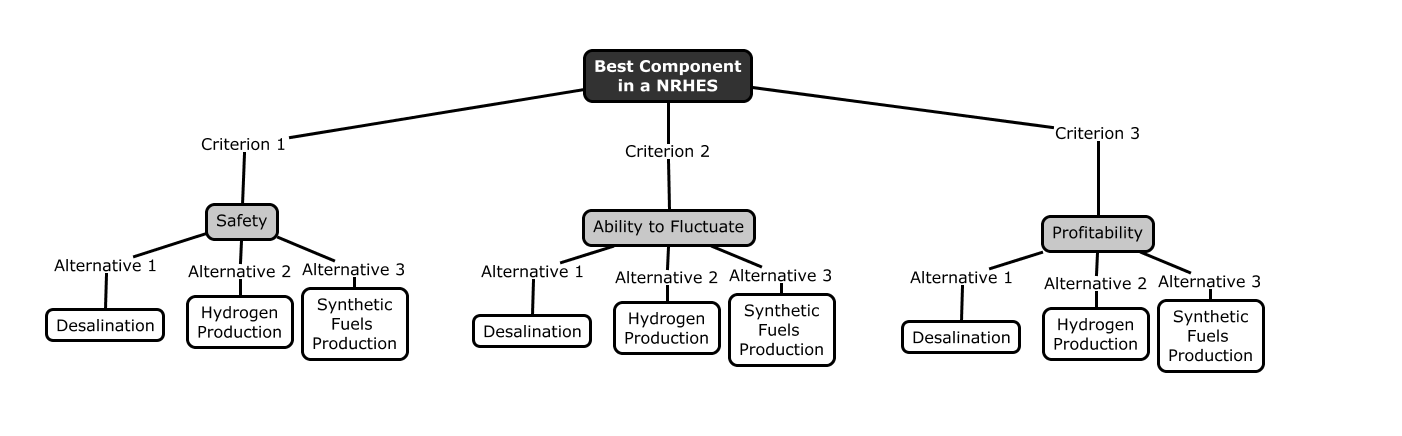
\includegraphics[width=0.9\textwidth]{AHP_hierarchy.PNG}
  \caption{A figure displaying the overall hierarchy of the industrial processes under evaluation for inclusion in the NRHES}
\end{figure}

The AHP provides not only insight into which is the best overall choice given the inputs and weights, but also which is the strongest candidate for each of the criterion. During the AHP process, before aggregating the values into one measurement, there are clear measurements of each of the alternatives in each of the criterion. The subjective nature of expert judgment as data requires a means of evaluation. As a check on the validity of the data,a traditional AHP measures the consistency of the values given by the experts using a Consistency Ratio, which needs to be less than .1, or 10\%, in order to be considered consistent. The Consistency Ratio compares the randomness of the expert judgments to a Random Consistency Index \cite{Saaty1987}.  If the consistency ratio is greater than .1, the data is judged to be too close to random.


\section{Fuzzy AHP}
Fuzzy logic applied to AHP takes into consideration the uncertainty inherent in a small number of expert opinions. Fuzzy AHP is an extension of the original AHP developed by Saaty in the 1970s \cite{Saaty1987}. Since Saaty's original development of AHP, multiple means of fuzzy AHP have emerged. Some notable fuzzy AHP approaches, as noted in \cite{Kahraman2010} include:
\begin{itemize}
\item Van Laarhoven and Pedrycz's approach from 1983 using triangular membership functions
\item Buckley's 1985 use of trapezoidal membership functions to determine fuzzy priorities
\item Cheng's 1997 approach focused on the grade value of the membership function.
\item Kahraman et al. generated a fuzzy weighted evaluation \cite{Kahraman2010}
\item Chang presented a new approach first determining triangular fuzzy numbers, then applying extent analysis method \cite{Chang1996}
\end{itemize}

 In the Buckley approach to fuzzy AHP, which is applied in this paper, $\alpha$ represents a value between zero and one reflecting the uncertainty.  Uncertainty is greatest when $\alpha$ is close to zero and least when close to one. As can be seen in the figure below, in a trapezoidal membership approach, the lower left point of the triangle, where $\alpha$ equals zero, is the minimum fuzzy number, the points making up the middle represent the most likely fuzzy number, and the point at a y value of zero on the right represents the maximum fuzzy number \cite{Pan2008}. The higher the fuzzy number on the x axis, the more important that criteria is, or the stronger the alternative.
\begin{figure}[h!]
  \caption{A figure displaying the meaning behind the membership function graph for the fuzzy numbers}
  \centering
  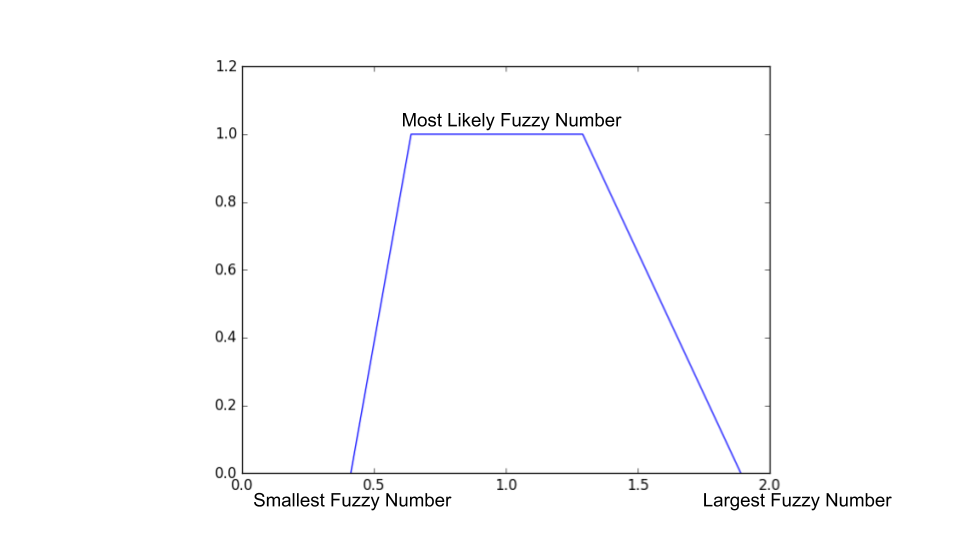
\includegraphics[width=0.9\textwidth]{Fuzzy_explaination.png}
\end{figure}

 As described in \cite{Kahraman2010}, after receiving the numbers from the decision makers, the fuzzy weight can be found by finding the geometric mean for each row in each of the AHP matrices:

 \begin{equation}
 z_i=[\prod_{j=1}^n t_{ij}]^{\frac{1}{n}}
 \end{equation}

 Where $t_{ij}=(a_{ij},b_{ij}, c_{ij}, d_{ij})$ which correspond to the fuzzy values in Table 1 below. $n$ is the number of values in each row.  For example, if three experts were taking a survey with three pairwise comparisons, there would be nine total answers in each row. To find the performance scores ($r$), first sum each of the geometric means in each row, then weight each of the values accordingly:

\begin{equation}
r_{ij}=(\frac{a_i}{d},\frac{b_i}{c},\frac{c_i}{b},\frac{d_i}{a})
\end{equation}

To find the fuzzy utility:

\begin{equation}
U_i=\sum_{j=1}^n w_j*r_{ij}
\end{equation}

where w is the weight found by the comparison of the importance of the various criteria to one another. To find the membership function $M(x)$, take the lowest value of the utility set and set the membership function to zero.  For the middle values of the utility set, the membership function is one. For all values greater than the greatest member of the utility set, the membership function is zero. For a utility set $(x_1,x_2,x_3,x_4)$

\begin{center}
\begin{tabular}{ |c|c| }
 \hline
 x & M(x)\\
 \hline
 $\leq x_1$  & 0 \\
 $\geq x_4$ & 0  \\
 $x_2 \leq x \leq x_3$ & 1  \\
 $x_1 \leq x \leq x_2$ & $\alpha \in [0,1]$\\
 $x_3 \leq x \leq x_4$ & $\alpha \in [0,1]$\\
 \hline
\end{tabular}
\end{center}

\begin{table}[h!]
\centering
\caption{Fuzzy Logic Value Mapping}
\label{Fuzzy values}
\begin{tabular}{|l|l|l|}
\hline
\textbf{Description }                                                           & \textbf{Values }       & \textbf{Inverse}           \\
\hline
Equal                                                                  & (1, 1, 1, 1)     & (1, 1, 1, 1)         \\
\hline
Equal Importance                                                       & (1/2, 3/4, 5/4, 3/2) & (2/3, 4/5, 4/3, 2)      \\
\hline
Weak Importance                                                        & (1, 3/2, 5/2, 3)   & (1/3, 2/5, 2/3, 1)   \\
\hline
Strong Importance                                                      & (2, 5/2, 7/2, 4)     & (1/4, 2/7, 2/5, 1/2) \\
\hline
\begin{tabular}[c]{@{}l@{}}Very Strong\\ Importance\end{tabular}       & (5, 11/2, 13/2, 7)     & (1/7, 2/11, 2/13, 1/5) \\\hline
\begin{tabular}[c]{@{}l@{}}Absolutely Strong\\ Importance\end{tabular} & (7, 15/2, 17/2, 9)     & (1/9, 2/17, 2/15, 1/7)\\
\hline
\end{tabular}
\end{table}

\section{Expert AHP Survey}
The objective for the expert AHP survey is to determine the optimal industrial process to include in a generic NRHES industrial park based on three criteria. The industrial process options are desalination, high temperature steam electrolysis, and synthetic fuel production. The criteria the options are judged on are ability to fluctuate, safety, and profitability. The optimal way to perform an Analytic Hierarchy Process (AHP) is to gather a group of experts with complementary specializations in a general field to discuss the relative values of various options under determined criteria. For example, performing an AHP to determine the optimal industrial process in a NRHES would best be done by gathering a group of experts in NRHESs with specialties in understanding each of the specific industrial processes. The group could discuss the relative values to give to each of the alternatives for a given criterion. Due to the struggles of getting a group of NRHES experts together in the same place, the values found for this research came from sending a survey to experts.  Other AHP evaluations employ similar methods\cite{Pan2008}. For this research, an expert is defined as someone who has published research or reports on NRHES.

	I chose the alternatives of desalination, hydrogen production, and synthetic fuels production due to their prominent role in research surrounding NRHES \cite{Bragg-Sitton2014,Locatelli2015,Kim2016,Bragg-Sitton2016,Garcia2016,Shropshire2011, Ruth2014,Bienvenu2015}.  I chose the criterion of ability to fluctuate as the industrial process in a NRHES will need to be able to fluctuate to adjust to change demand as well as the dynamic generation from the industrial process.  I chose the criterion of safety due to the inherent need for safety, especially within the context of the nuclear safety culture.  Safety underlies both the characteristic of ability to fluctuate and profitability. If the industrial process is not safe, it will not run, and therefore the other two characteristics are negligible. I chose profitability as clearly the whole NRHES will need to be profitable in order to continue to run.  The industrial process provides a secondary source of income  increasing the overall profitability of the system as a whole.

	I chose the alternatives of desalination, hydrogen production, and synthetic fuels production due to their prominent role in research surrounding NRHES \cite{Bragg-Sitton2014,Locatelli2015,Kim2016,Bragg-Sitton2016,Garcia2016,Shropshire2011, Ruth2014,Bienvenu2015}.  I chose the criterion of ability to fluctuate as the industrial process in a NRHES will need to be able to fluctuate to adjust to change demand as well as the dynamic generation from the industrial process.  I chose the criterion of safety due to the inherent need for safety, especially within the context of the nuclear safety culture.  Safety underlies both the characteristic of ability to fluctuate and profitability. If the industrial process is not safe, it will not run, and therefore the other two characteristics are negligible. I chose profitability as clearly the whole NRHES will need to be profitable in order to continue to run.  The industrial process provides a secondary source of income  increasing the overall profitability of the system as a whole.

There were five experts who completed the Analytic Hierarchy Process for a Nuclear Renewable Hybrid Energy System survey. Due to the small number of experts included in the survey, a fuzzy systems approach has been applied to the AHP. Tsyganok et al. determined that the expert competence should always be taken into consideration, especially when there are less than 50 experts included in the evaluation \cite{Tsyganok2012}. Thus in this case a fuzzy approach is clearly applicable due to the low number of responses.

 For this research, the same NRHES with only the industrial process switched out will be compared. The assumptions for this research include:
\begin{itemize}
\item The process used for hydrogen production is high temperature steam electrolysis with thermal as well as electrical coupling to the nuclear power plant
\item  The process for desalination is thermal desalination through distillation directly using heat from the nuclear power plant
\item The synthetic fuel process is a Fischer-Tropsch method using coal as the hydrocarbon source
\item Each of the processes consumes the same amount of heat from the nuclear power plant
\item All of the industrial processes are thermally coupled
\item Regional accessibility of feedstocks for each of the industrial processes are the same
\item Regional transportation costs are the same
\item Regulatory and taxation costs are the same
\end{itemize}

As can be seen in Table 2 below, the scale for the answers for the second part of the question ranged from two to  nine.  In the initial question the expert determines which of the alternatives better fits the criteria.  If the two alternatives were judged to equally answer the question, then a value of 1 was assigned to the relative importance of both. Table 3.5 displays the relative values for each of the characteristics considered in the AHP. The values are chosen on a scale of one to nine, with the industrial process strongly reflecting that characteristic receiving a nine and the characteristic relatively less reflecting those characteristics receiving appropriate smaller numbers. While the safety of the system is in reality the most important characteristic, as it is the foundation which the economic and grid reliability characteristics rely on, the safety issues are the most easy to mitigate and the most well known.

\begin{table}[h!]
\centering
\caption{Example of questions given in the Expert AHP survey}
\label{my-label}
\begin{tabular}{l}
Questions included in the expert AHP survey:                                                                                   \\ \hline
\multicolumn{1}{|l|}{\begin{tabular}[c]{@{}l@{}}Q1a: Do you think that the ability to fluctuate,is more important\\ than profitability of an industrial process?\\ Q1b: From 2 to 9, how would you compare the importance of \\ safety of an industrial process to the ability of the industrial process to fluctuate?\\ Q2a: Do you think that the ability to fluctuate,is more important than \\ profitability of an industrial process?\\ Q2b: From 2 to 9, how would would you compare the importance \\ of safety of an industrial process to the ability of the industrial process to fluctuate?\end{tabular}} \\ \hline
\end{tabular}
\end{table}

\begin{table}[h!]
\centering
\caption{AHP Scale Description}
\label{my-label}
\begin{tabular}{|l|l|l|}
\hline
Quantitative Value & Explanation                                                                                                                              & Verbal Judgement                                                        \\ \hline
1                  & \begin{tabular}[c]{@{}l@{}}They are equally important \\ or equally meet the criterion\end{tabular}                                      & Equally more important                                                  \\ \hline
2                  & \begin{tabular}[c]{@{}l@{}}Experience and judgement \\ favor one alternative over \\ the other by a small margin\end{tabular}            & Weakly more important                                                   \\ \hline
3                  & \begin{tabular}[c]{@{}l@{}}Experience and judgement \\ moderately favor one \\ alternative over the other\end{tabular}                   & Weakly more important                                                   \\ \hline
4                  & \begin{tabular}[c]{@{}l@{}}Experience and judgement \\ clearly favor one \\ alternative over the other\end{tabular}                      & Strongly more important                                                 \\ \hline
5                  & \begin{tabular}[c]{@{}l@{}}Experience and judgement \\ strongly favor one \\ alternative over the other\end{tabular}                     & Strongly more important                                                 \\ \hline
6                  & \begin{tabular}[c]{@{}l@{}}Practice suggests moderate\\ preference for one alternative \\ over the other\end{tabular}                    & \begin{tabular}[c]{@{}l@{}}Very strongly more\\ important\end{tabular}  \\ \hline
7                  & \begin{tabular}[c]{@{}l@{}}One alternative is favored \\ very strongly over the other \\ and has been shown in practice\end{tabular}     & \begin{tabular}[c]{@{}l@{}}Very strongly more \\ important\end{tabular} \\ \hline
8                  & \begin{tabular}[c]{@{}l@{}}It is fairly clear that, in practice\\ one alternative is better than the \\ other\end{tabular}               & \begin{tabular}[c]{@{}l@{}}Absolutely more \\ important\end{tabular}    \\ \hline
9                  & \begin{tabular}[c]{@{}l@{}}The evidence favoring one \\ alternative over the other is of\\ the highest possible affirmation\end{tabular} & \begin{tabular}[c]{@{}l@{}}Absolutely more \\ important\end{tabular}    \\ \hline
\end{tabular}
\end{table}

\section{Results and Discussion}
As can be seen in table 4, the utility set values which comprise the membership function are highest for desalination. The utility set generates the weighted value for each of the alternatives using the geometric mean method discussed above. As the higher the utility the greater the value, desalination ranks highest of the options for an industrial process given the criteria. As can be seen in Table 5, safety clearly was prioritized.  Due to the high value placed on safety, and the sense that desalination is safer than the alternatives, it follows that it has a greater fuzzy number. Clearly, the heavy weight placed on safety played a major role in determining the outcome.

While AHP provides a means to compare various options and criteria, it is limited by not including vital information surrounding when a certain standard has been met. In the case of this research, safety and flexibility standards could have been fully met by all of the industrial processes. Safety, instead of being a relative point of comparison, may be better treated as a set of standards to be achieved, such as those presented in the International Organization for Standardization standards for cogeneration \cite{ISO2017}. While desalination is perceived to be a safer industrial process, that does not mean that a synthetic fuel upgrading system or a high temperature steam electrolysis plant is unsafe to couple to a nuclear power plant. The fact that desalination is perceived as safer and more able to fluctuate becomes negligible at that point. AHP is a beneficial tool when determining the relative value between alternatives.  For example, profitability is a valuable characteristic to compare on relative terms.

NRHESs are difficult systems to have a fully developed sense of expertise surrounding. Due to the industrial parks including different components as well as the importance of including technical, economic, and political variables in the decision making. While an AHP is a valuable tool because it is able to include a variety of characteristics from different disciplines, there need to be experts representing each of the disciplines. Furthermore, the more experts included in the survey, the stronger the data and the more likely a valid conclusion can be drawn from the data.
\begin{table}[h!]
\centering
\caption{Utility Set values for each of the industrial processes}
\label{my-label}
\begin{tabular}{|l|l|}
\hline
\begin{tabular}[c]{@{}l@{}}Industrial \\ Process\end{tabular} & Utility Set               \\ \hline
Desalination                                                  & (0.412, 0.641, 1.291, 1.891) \\ \hline
\begin{tabular}[c]{@{}l@{}}Hydrogen\\ Production\end{tabular} & (0.029, 0.047, 0.084, 0.136) \\ \hline
\begin{tabular}[c]{@{}l@{}}Synthetic \\ Fuels\end{tabular}    & (0.086, 0.128, 0.265, 0.437) \\ \hline
\end{tabular}
\end{table}




\begin{table}[h!]
\centering
\caption{Performance Scores of Safety for the various industrial processes included}
\label{my-label}
\begin{tabular}{|l|l|}
\hline
Industrial Process                                                    & Safety Performance Score     \\ \hline
Deslination                                                           & (0.309,0.424, 0.708, 0.917)  \\ \hline
\begin{tabular}[c]{@{}l@{}}Hydrogen \\ Production\end{tabular}        & (0.118, 0.162 ,0.277 ,0.390) \\ \hline
\begin{tabular}[c]{@{}l@{}}Synthetic Fuels \\ Production\end{tabular} & (0.139, 0.181, 0.317, 0.459) \\ \hline
\end{tabular}
\end{table}

\begin{table}[h!]
\centering
\caption{Ability to Fluctuate Performance Scores for the various industrial processes included}
\label{my-label}
\begin{tabular}{|l|l|}
\hline
\begin{tabular}[c]{@{}l@{}}Industrial \\ Process\end{tabular} & \begin{tabular}[c]{@{}l@{}}Ability to Fluctuate \\ Performance Scores\end{tabular} \\ \hline
Desalination                                                  & (0.328, 0.436, 0.687, 0.868)                                                       \\ \hline
\begin{tabular}[c]{@{}l@{}}Hydrogen\\ Production\end{tabular} & (0.183, 0.234, 0.365, 0.496)                                                       \\ \hline
\begin{tabular}[c]{@{}l@{}}Synthetic \\ Fuels\end{tabular}    & (0.104, 0.129, 0.199, 0.262)                                                       \\ \hline
\end{tabular}
\end{table}

\begin{table}[h!]
\centering
\caption{Profitability Performance Scores for the various industrial processes included}
\label{my-label}
\begin{tabular}{|l|l|}
\hline
\begin{tabular}[c]{@{}l@{}}Industrial \\ Process\end{tabular} & \begin{tabular}[c]{@{}l@{}}Profitability \\ Performance Scores\end{tabular} \\ \hline
Desalination                                                  & (0.110, 0.146, 0.206, 0.271)                                                \\ \hline
\begin{tabular}[c]{@{}l@{}}Hydrogen\\ Production\end{tabular} & (0.210, 0.282, 0.425, 0.544)                                                \\ \hline
\begin{tabular}[c]{@{}l@{}}Synthetic \\ Fuels\end{tabular}    & (0.297, 0.383, 0.602, 0.805)                                                \\ \hline
\end{tabular}
\end{table}

\begin{table}[h!]
\centering
\caption{Fuzzy weights of each of the criteria. Clearly, safety is weighted most heavily and ability to fluctuate is weighted the least}
\label{my-label}
\begin{tabular}{|l|l|}
\hline
\begin{tabular}[c]{@{}l@{}}Industrial \\ Process\end{tabular}   & Fuzzy Weights                \\ \hline
Safety                                                          & (0.552, 0.637, 0.806, 0.919) \\ \hline
\begin{tabular}[c]{@{}l@{}}Ability to \\ Fluctuate\end{tabular} & (0.057, 0.069, 0.079, 0.095) \\ \hline
Profitability                                                   & (0.159, 0.185, 0.237, 0.286) \\ \hline
\end{tabular}
\end{table}

As can be seen in figure 3.3 below, the membership function for desalination is clearly the highest.  As can be seen in the performance score table, synthetic fuels upgrading was perceived as both safer and more profitable than hydrogen production, resulting in the generally higher membership function values for the synthetic fuels production. As discussed above, it is possible that all three industrial processes meet a certain threshold of safety and flexibility. In terms of profitability, synthetic fuels upgrading was the highest, followed by hydrogen production, with desalination coming in at a distant third as can be seen in the profitability performance score table.

\begin{figure}[h!]
  \caption{A figure displaying the fuzzy utility function for the three industrial processes.  The furthest to the right has the highest importance. Clearly Desalination has the greatest fuzzy number.}
  \centering
  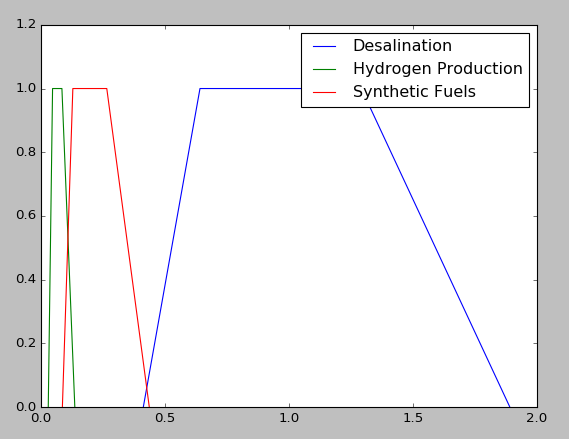
\includegraphics[width=0.5\textwidth]{membership.PNG}
\end{figure}


\begin{table}[h!]
\centering
\caption{AHP Survey answers for determining the relative importance of different criteria}
\label{my-label}
\begin{tabular}{|l|l|l|l|l|l|}
\hline
\begin{tabular}[c]{@{}l@{}}Pairwise \\ Criteria\end{tabular}                       & 1st Expert       & 2nd Expert       & 3rd Expert & 4th Expert       & 5th Expert       \\ \hline
\begin{tabular}[c]{@{}l@{}}Safety vs \\ Ability to \\ Fluctuate\end{tabular}       & Safety: 6        & Safety: 9        & Safety: 8  & Safety: 6        & Safety: 7        \\ \hline
\begin{tabular}[c]{@{}l@{}}Safety vs \\ Profitability\end{tabular}                 & Safety: 8        & Safety: 8        & Safety: 8  & Equal            & Safety: 7        \\ \hline
\begin{tabular}[c]{@{}l@{}}Ability to \\ Fluctuate\\ vs Profitability\end{tabular} & Profitability: 8 & Profitability: 7 & Equal      & Profitability: 8 & Profitability: 4 \\ \hline
\end{tabular}
\end{table}

\newpage
\section{Conclusion and Future Work}

AHP should be used early in the design and decision making process to determine the best options given a set of criteria. Unlike other systems which can be compared to experimental setups, AHP evaluates systems which cannot have large scale experiments. Given the criteria of safety, ability to fluctuate, and profitability a multi-stage flash distillation system appears to be the best choice in a generic setup when compared with synthetic fuels upgrading and hydrogen production from high temperature steam electrolysis. In future work applying AHP to NRHES configurations, considerations such as access to feedstocks, for example water and hydrocarbons, will likely play a large role in determining the industrial process incorporated.

 Future work on applying AHP to NRHES would include many more criteria, subcriteria, and alternatives which are important to evaluate on a relative basis.  Criteria such as emissions, a key driver for NRHES, would be important to consider before determining the optimal industrial process for a given industrial park. Other criteria such as likely regulatory barriers and state of development of the industrial process technology would also be valuable to include in future research.

\chapter{Thermal Versus Electrical Coupling}
From the literature review on NRHES, a notable gap in the current research is modeling the benefits gained from thermally coupling systems as compared to electrically coupling. The major drawback of thermally coupling any industrial process to a nuclear power plant is the increase in complexity. While there are cases of thermal coupling of nuclear power plants internationally; in Norway, Switzerland, Germany, and Canada \cite{Verfondern};  there have never been any nuclear thermal couplings thus far in the United States.  The low level state of development as well as the lack of experimental data in the United States suggest a demand for rigorous technical work.  There are concerns surrounding the regulatory oversight with a thermally coupled NRHES and whether it falls under the Nuclear Regulatory Commission's umbrella. The efficiency benefits would have to be greater than the costs associated with thermal coupling and co-location.  An exergy analysis of both the electrically coupled and thermally coupled industrial processes provides a quantitative measure of the benefits of thermally coupling. As the fuzzy AHP analysis concluded that the optimal industrial process; given the requirements of safety, ability to fluctuate, and profitability; is desalination, the exergy evaluation will focus on two desalination systems.  Multi-stage flash (MSF) distillation is the thermally coupled desalination system included in this analysis. For comparison, an electrically coupled basic reverse osmosis system is also included.


\section{Exergy Analysis}
The exergetic efficiency concept, also known as second law efficiencies, can be applied to all of the various components involved in the coupling of a Nuclear Renewable Hybrid Energy system. An exergy analysis determines the energy available in a system to do work. The exergy analysis can then be combined with an economic analysis determining where exergy losses are most costly. For this project, the components in the exergetic analysis will be applied to include the aspects of a Rankine Cycle as well as the multi stage flash distillation system. In order to compare a thermally coupled industrial process with an electrically coupled desalination process, the exergy analysis for the electrically coupled plant will stop at the generation of the electricity. In order to evaluate the exergetic efficiency of nuclear as compared to other resources for electricity production, an exergetic analysis will be done on coal plants as well as a concentrated solar generation system.

  Boldon et. al. has already performed an initial exergy analysis on a nuclear hybrid energy system, assuming a Small Modular Reactor (SMR) \cite{Boldon}. Boldon et. al. discusses the value of combining exergy and economics to analyze costs associated with exergetic losses.  Boldon et. al. analyzes a steady state system providing a constant grid output of 245 MWe.  The nuclear plant is both thermally and electrically coupled to a High Temperature Steam Electrolysis industrial process. After performing the thermodynamic exergy analysis, Boldon et. al. incorporates costs of resources and operations thereby able to assign a unit exergetic cost to each of the components in the system.

 An exergetic analysis of the Kalundborg industrial ecosystem evaluates the streams going into and out of the Asnaes power plant \cite{Valero2012}.  Valero et. al. contrast the exergy of the coupled system with an uncoupled system. As can be seen in figure below, the Kalundborg industrial ecosystem is comprised of the Statoil refinergy, the Asnaes coal power plant, the Novo Group pharmaceutical company, district heating for the local people, the Gyproc plasterboard manufacturer, as well as a fish farm, and  the Aalborg Portland cement company. The major exergetic gains for the system come from sharing the process natural gas, the district heating, heating the fish farm, and using clinker (a coal plant byproduct) to produce cement \cite{Valero2012}. The overall reduction in irreversibilities annually from coupling the systems at Kalundborg amount to approximately 1476 GWh/year, the equivalent of the annual production of a 170.235 MW power plant. An analysis which compares the exergy of a coupled system with the seperate industrial processes provides great insight into what are the thermodynamic and economic benefits of co-locating processes.

 The exergy analysis done here will assume a the Palo Verde Rankine power cycle and a multi-stage flash distillation system.  First, I will evaluate the use of waste heat from both a nuclear power plant and a natural gas plant.  Then I will evaluate the direct heat from the reactor for both a nuclear power plant and a natural gas plant. An exergy analysis really evaluates where there are irreversibilities in a system.  In the case of the thermally coupled systems, the irreversibilities associated with the electrical generation and reconversion into heat do not exist.  While there are still losses in a thermally coupled system, primarily associated with having to pump the water, there are not the losses associated with the conversion of energy from heat to electrical and back.


\section{Multi-Stage Flash Distillation}
As the NRHES evaluated for this thesis includes a \ac{msf} distillation system, I will include a brief review of a previous MSF distillation exergy analysis. Kahraman et. al. perform an exergy analysis on a large MSF plant \cite{Kahraman2005}.  Multi-Stage Flash distillation only requires heat at about 100 degrees Celsius, making it possible to use the waste heat from a nuclear power plant to desalinate the water. In the exergy analysis, Kahraman et. al. takes the temperature of the salinated water to be the dead state, making the initial exergy zero. The exergy analysis includes finding the exergy of the heat exchanger, of four pumps in the system, as well as the difference in exergies between the incoming water and the exiting stream.

\begin{figure*}
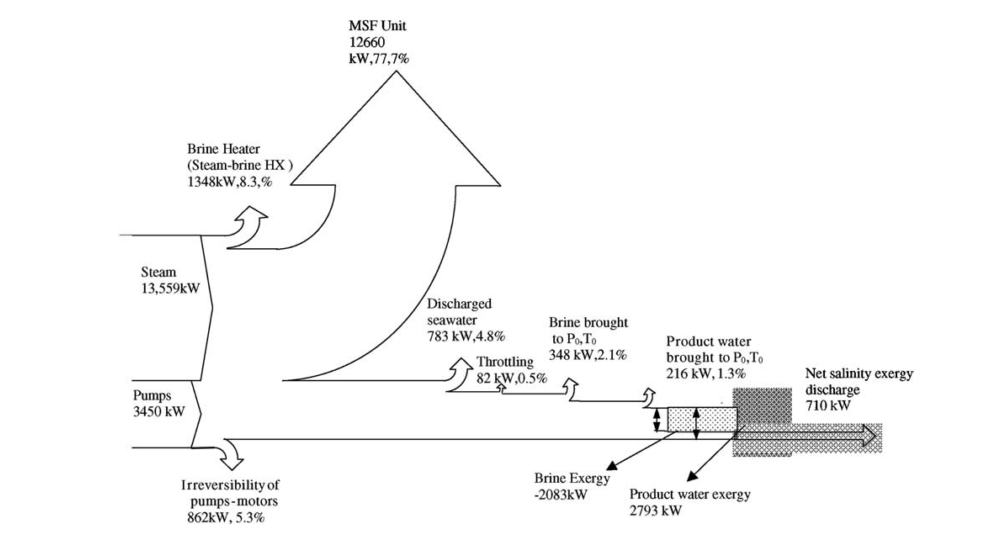
\includegraphics[width=.7\textwidth]{MSF_exergy.PNG}
\caption{\small \sl The Multi-Stage Flash exergy analysis diagram showing where exergy is lost in the system}
\end{figure*}


	Assuming a closed system, the exergy rate balance is:
\begin{equation}
\frac{dE}{dt}=\Sigma_j(1-\frac{T_0}{T_j})\dot{Q}_j-(\dot{W}-p_0*\frac{dV}{dt})-
\end{equation}

A quick exergy analysis comparing electrical coupling and thermally coupling would only evaluate the losses associated with the power conversion.  The quick exergy analysis would not permit an evaluation of how much product, and the quality of the product, produced in each instance. In order to do an economic analysis, evaluating the \$/exergy, requires knowing the amount of product sold as well as the value of the product.

Multistage flash distillation (MSF) is the most common thermal desalination system. In an MSF system, briny water is flash evaporated, then condensed repeatedly in order to remove unwanted particulates. MSF is able to produce clean water in large quantities, with plants in Saudi Arabia and the United Arab Emirates having capacities of 600,000-880,000 $m^3/day$ \cite{El-Dessouky2016}. The general idea of how an MSF system works is briny or sea water is passed through a series of chambers, each with successively lower temperature and pressure.  The water is quickly flashed, or vaporized.  The water, without the brine, is then condensed forming freshwater.  There are a wide range of stages, depending on the concentration of the feedwater brine and the desired state of purity for the freshwater.


\subsection{Drinking Water Standards}
The Safe Drinking Water Act of 1974 gives the \ac{epa} the authority to determine safe drinking water standards.

Energy balance equation for a single pass Multi-Stage Flash Desalination plant.

\begin{equation*}
\begin{aligned}
\frac{dH_{bj}}{dt}=[B_{bj-1}h_{bj-1}-B_{bj}h_{bj}-(B_{bj-1}-B_{bj}-H_{bj}A_{bj}\frac{d\rho_{bj}}{dt}h_{vj})]\\
*[\frac{1}{A_{bj}\rho_{bj}(h_{bj}-h_{vj})}] (-H_{bj}*\frac{h_{bj}}{\rho_{bj}(h_{bj}-h_{ij})}*\frac{d\rho_{bj}}{dt})-\frac{H_{bj}}{h_{bj}-h_{vj}}\frac{dh_{bj}}{dt},
\end{aligned}
\end{equation*}

Mass Balance of the Distillate:
\begin{equation*}
\frac{dH_{dj}}{dt}=\frac{1}{A_{dj}{\rho_{dj}}}*[B_{i-1}*D_{i-1}-B_j-D_j]-\frac{H_{dj}d\rho_{dj}}{\rho_{dj}*dt}-\frac{A_{bj}\rho_{bj}dH_{bj}}{A_{dj}\rho_{dj}dt}-\frac{H_{bj}A_{bj}d\rho_{bj}}{A_{dj}\rho_{dj}dt}
\end{equation*}

Salt balance in the flashing brine:

In a multi-stage flash system, it is important to keep the temperature relatively low, no greater than 120 \degree C in order to minimize fouling. This makes multi-stage flash a perfect industrial process to couple to the waste heat of a power plant.

\begin{table}[]
\centering
\caption{The Components of Briny Groundwater in Arizona (name the well)}
\label{my-label}
\begin{tabular}{|l|l|}
\hline
Material                                                   & Mole Percent \\ \hline
Calcium                                                    & 0.00732      \\ \hline
Magnesium                                                  & 0.00511      \\ \hline
Sodium                                                     & 0.0324       \\ \hline
\begin{tabular}[c]{@{}l@{}}Sulfur \\ Trioxide\end{tabular} & .00947       \\ \hline
Water                                                      & 99.9         \\ \hline
\end{tabular}
\end{table}

\section{Palo Verde Power Cycle}

One unit at the Palo Verde Nuclear Generating Station is considering a reverse osmosis system both to fluctuate the load sent to the grid as well as to produce water. For the power cycle, the assumed values will be in regard to Palo Verde.

The turbine-generator load change characteristics are
compatible with the restrictions imposed by or on the
nuclear steam supply system (NSSS). The NSSS is
capable of accepting a step load change of 10\% and ramp
load change of 5\% per minute over the load range of 15
to 100\%.

From Palo Verde UFSAR
"The feedwater pumps discharge the total feedwater flow through
the high-pressure feedwater heaters to the steam generators."

\begin{table}[h!]
\centering
\caption{Palo Verde Reactor Core Thermohydraulic Values}
\label{my-label}
\begin{tabular}{|l|l|l|}
\hline
\textbf{Reactor Core Values} & \textbf{Value Given in FSAR} & \textbf{Units in Model}        \\ \hline
Reactor Outlet Temperature   & 653 \degree F & 345 \degree C   \\ \hline
Reactor Inlet Temperature    & 568 \degree F & 297.8 \degree C \\ \hline
Mass Flow                    & $164.0x10^6\frac{lb}{hr}$    & $20663.6\frac{kg}{s}$          \\ \hline
Pressure                     & 2250 psia                    & 15.513 MPa                     \\ \hline
Power Generation             & 3800 MWt                     & 3800 MWt                       \\ \hline
\end{tabular}
\end{table}

\begin{table}[h!]
\centering
\caption{Palo Verde Main Steam Flow Power Cycle}
\label{my-label}
\begin{tabular}{|l|l|l|}
\hline
\textbf{Power Cycle Values} & \textbf{Value Given in FSAR}  & \textbf{Units in Model}          \\ \hline
Steam Temperature at HX     & 552.9 \degree F                & 289.4 \degree C                   \\ \hline
Maximum Quality             & 0.25                          & 0.25                             \\ \hline
Mass Flow                   & $17.2-18.1x10^6\frac{lb}{hr}$ & $2154.56-2280.56 \frac{kg}{sec}$ \\ \hline
Pressure                    & 1070 psia                     & 7.377 MPa                        \\ \hline
Power Generation            & 3800 MWt                      & 3800                             \\ \hline
\end{tabular}
\end{table}

\begin{table}[]
\centering
\caption{Palo Verde Main Condenser Values}
\label{my-label}
\begin{tabular}{|l|l|l|}
\hline
\textbf{Main Condenser Values}                                                       & \textbf{Value Given in FSAR}       & \textbf{Units in Model}          \\ \hline
Feedwater temperature                                                                & 450 degree F                       & 232.22  degree C                 \\ \hline
Total condenser duty                                                                 & $9.04x10^9\frac{Btu}{hr}$          & 2649.36 MW                       \\ \hline
\begin{tabular}[c]{@{}l@{}}Circulating water design\\ flow to condenser\end{tabular} & $560,000\frac{gal}{min}$           & $4233.53 \frac{kg}{s}$           \\ \hline
\begin{tabular}[c]{@{}l@{}}Exhaust Steam to \\ Condenser\end{tabular}                & $9,303,000-9,361,830\frac{lb}{hr}$ & $2154.56-2280.56 \frac{kg}{sec}$ \\ \hline
Pressure                                                                             & 3.5 in.Hg abs                      & 11.8524 kPa                      \\ \hline
\end{tabular}
\end{table}

\begin{table}[h!]
\centering
\caption{Pump Values for Palo Verde from U-FSAR\cite{Rogalski2007}}
\label{my-label}
\begin{tabular}{|l|l|l|l|l|l|l|}
\hline
\multicolumn{1}{|c|}{\textbf{Pumps}}                                  & \multicolumn{1}{c|}{\textbf{Description}}                                                                                              & \multicolumn{1}{c|}{\textbf{\begin{tabular}[c]{@{}c@{}}Operating\\  Pressure\\ (psia)\end{tabular}}} & \multicolumn{1}{c|}{\textbf{\begin{tabular}[c]{@{}c@{}}Temp\\ (F)\end{tabular}}} & \multicolumn{1}{c|}{\textbf{\begin{tabular}[c]{@{}c@{}}Design \\ Capacity \\ (gal/min)\end{tabular}}} & \multicolumn{1}{c|}{\textbf{\begin{tabular}[c]{@{}c@{}}Design \\ head (ft)\end{tabular}}} & \multicolumn{1}{c|}{\textbf{\begin{tabular}[c]{@{}c@{}}Motor \\ Rating\\ (hp)\end{tabular}}} \\ \hline
\begin{tabular}[c]{@{}l@{}}Reactor\\ Coolant \\ Pumps\end{tabular}    & \begin{tabular}[c]{@{}l@{}}4, Vertical single \\ stage centrifugal \\ with bottom\\ suction and \\ horizontal\\ discharge\end{tabular} & 2250                                                                                                 & 564.5                                                                            & 111400                                                                                                & 363                                                                                       & 12000                                                                                        \\ \hline
\begin{tabular}[c]{@{}l@{}}Reactor Makeup \\ Water Pumps\end{tabular} & 2                                                                                                                                      & 200 psig                                                                                             & 200                                                                              & 165                                                                                                   & 300                                                                                       &                                                                                              \\ \hline
\begin{tabular}[c]{@{}l@{}}Aux \\ Feedwater \\ Pumps\end{tabular}     & 1                                                                                                                                      & 1270                                                                                                 & 180                                                                              & 650                                                                                                   & 3280                                                                                      & 1190.2 BHP                                                                                   \\ \hline
\end{tabular}
\end{table}

Annually, Palo Verde uses approximately 75,700 acre feet per year.  To ensure that Palo Verde continues to have sufficient water for operations coming from groundwater resources, the model is determining the heat resources required to meet 20\% of the annual water demand.  Thus, the system needs to be able to produce approximately 15,140 acre feet per year, or 1.728 acre feet per hour.

\section{Aspen HYSYS}

Aspen HYSYS is a process simulation software used primarily by the oil and gas industry. In this model, Aspen HYSYS calculates the overall thermodynamic and mass flow values of the Palo Verde Power Cycle as well as the multistage flash distillation process.  The values for the Palo Verde Power Cycle were found in the updated Final Safety Analysis Report (U-FSAR) for the plant.

\section{Results}

For the initial results found from using waste process heat, the pressure of the distillation inlet was manipulated to permit 100\% of the water flowing through the condenser to go through the Multi Stage Flash Distillation unit.  The temperate needed to be kept at 120 degrees and below in order to avoid fouling.

\begin{landscape}
\begin{table}[h!]
\centering
\caption{My caption}
\label{my-label}
\begin{tabular}{|l|l|l|l|l|l|l|l|l|l|}
\hline
\textbf{\begin{tabular}[c]{@{}l@{}}Temp of \\ Water from \\ Condenser \degree C\end{tabular}} & \textbf{\begin{tabular}[c]{@{}l@{}}Temp of\\ Water into\\ Distillation\\ System \degree C\end{tabular}} & \textbf{\begin{tabular}[c]{@{}l@{}}Pressure of \\Distillation\\ Inlet (kPa)\end{tabular}} & \textbf{\begin{tabular}[c]{@{}l@{}}Percent of \\ Condenser\\ Water to MSF\\ Distillation unit\end{tabular}} & \textbf{\begin{tabular}[c]{@{}l@{}}Mass Flow \\ Distillate\\ (kg/s)\end{tabular}} & \textbf{\begin{tabular}[c]{@{}l@{}}Mass Flow \\ Brine\\ (kg/s)\end{tabular}} & \textbf{\begin{tabular}[c]{@{}l@{}}Heat/Spec \\ Error\end{tabular}} & \textbf{\begin{tabular}[c]{@{}l@{}}Pumps \\ Power\end{tabular}} & \textbf{\begin{tabular}[c]{@{}l@{}}Heat Flow\\ In Brine\\ (MW)\end{tabular}} & \textbf{\begin{tabular}[c]{@{}l@{}}Distillate\\ Heat Flow\\ (MW)\end{tabular}} \\ \hline
120  & 120  &  107.8 &   100\% & 1694 & 2635  & 0.006958 & 0 & 255.2 &  8000 \\ \hline
110 & 110.1 & 107.8 & 100\% & 1745 & 2688 & 0.009954 & 0 & 318.3 & 7687\\ \hline
100 & 100 & 231 & 100\% & 12740 & 19340 & 0.006015 & 5.347 & &  \\ \hline
95  & 95.02  & 231.0 & 100\%  & 13110 & 21000 & 0.000934 & & 44280 & 43340\\ \hline
90 & 90.02 & 231.0 & 100\% & 13980 & 22440 & 0.000164 &  & 46960 & 47260\\ \hline
85 & 85.02 & 231 & 100\% & 14970                                                                                      &                                                                                       &                                                                     &                                                                & 51310                                                                        & 50670                                                                          \\ \hline
20                                                                                                                  & 20.01                                                                                                                         & 231                                                                                     &                                                                                                             &                                                                                            &                                                                                       &                                                                     &                                                                & 965400                                                                   & 791300                                                                         \\ \hline
\end{tabular}
\end{table}
\end{landscape}

Note that at the higher temperatures there is less mass flow in both the brine and the distillate.  There is less mass flow in general due to less water being able to be heated to 120 \degree C.

\section{Notes to Self}


Energy efficiency is often characterized as using less energy to perform the same tasks.
From discussion with Dr. Cristian Rabiti on 2/22/2018:

- Prove electrical coupling only beneficial when lag (delayed response) is included.  Show the marginal cost gains become zero when factoring in the gains from the nuclear power plant not having to curtail as compared to the marginal costs of running the industrial process. Calculate the NPV as equaling zero between the industrial process and the NPP.

-Calculate the cost of exergy for coal, nuclear, natural gas.  Demonstrate that, in terms of exergy, there is a lot more to gain from thermally coupling as opposed to electrically coupling.

Ways that thermal coupling can increase efficiency of industrial processes:
\begin{itemize}
\item Desalination - pre heating for an RO plant, direct heating for MED and MSF plants
\end{itemize}



\chapter{Future Work}
\begin{itemize}
\item Include Fluctuation in a more dynamic manner instead of a qualitative assessment of the differences between MSF and RO desalination.
\end{itemize}



\section{Summary Remarks}


\section{Examples of acronyms}
\ac{epri}
\ac{nfcs}
\ac{lcoe}
\ac{ece}
\ac{ahp}

% --------------------------------------------------------------------------
% --  --


% --------------------------------------------------------------------------
% -- Summary and Conclusions --
\chapter{Summary and Conclusions}
\label{Chapter:SummaryAndConclusions}

Example summary and conclusions. You can refer to chapters and sections using their label, e.g Chapter %\ref{Chapter:Introduction}.

% --------------------------------------------------------------------------
% -- References --

\clearpage
\renewcommand\bibname{References} % Relabels bibliography title as "REFERENCES"
\addcontentsline{toc}{chapter}{\textsc{\bibname}} % Adds to table of contents
\bibliographystyle{plain}  % Sets style, plain is fine for this
\bibliography{example-bib-file.bib}  % Name of bibliography file containing your references. It is best practice to have a separate file, as it makes it easier to share your references, make derivative works, or use the references from a prior work (e.g a prior paper that your thesis work is building on).

% Examples of citing GitHub repositories:
%   http://academia.stackexchange.com/a/14015
%   https://github.com/blog/1840-improving-github-for-science
%   https://guides.github.com/activities/citable-code/
%   https://github.com/GhostofGoes/uidaho-masters-thesis/
%   Wait, that last one is recursive...oh no. RIP poorly programmed web crawling spider.




% --------------------------------------------------------------------------
% -- Appendices --
\clearpage
\appendix  % Marks start of appendices

% Appendices are done as LaTeX chapters
\chapter{Your fist appendix}
Fuzzy Analytic Hierarchy Code:

import numpy
import csv
import matplotlib.pyplot as plt

\#Functions
def GeometricMean(LineList, Spot):
    values = [x[Spot] for x in LineList]
    GeoMean=1
    for i in range(len(LineList)):
        GeoMean=GeoMean*values[i]
    return(GeoMean**(1/len(LineList)))

def PerformanceScores(a, b, c, d):
    \# The number of rows in each matrix will always be three, so I am hard coding it in
    PS=[0]*3
    for x in range(3):
        PS[x]=[a[x]/sum(d), b[x]/sum(c), c[x]/sum(b), d[x]/sum(a)]
    return(PS)

\#Weight all of the performance score values
\#Add all of the values in the individual locations together
\#Return the utility function for safety, ability to fluctuate, and profitability
def WeightPS($r_{ij}$, weight):
    weightedPS=[0]*len($r_{ij}$)
    for i in range(len($r_{ij}$):
        weightedPS[i]=[a*b for a,b in zip($r_{ij}$[i],weight[i])]
        print(i,$r_{ij}$[i])
    Desal=weightedPS[0]
    HProd=weightedPS[1]
    SynFuel=weightedPS[2]
    return(Desal, HProd, SynFuel)

def Utility(A, B, C):
    utility=[0]*len(C)
    for x in range(len(C)):
        utility[x] = A[x]+B[x]+C[x]
    return(utility)




\#CONSTANTS AND INPUT
\#1 corresponds to equally important
\#2-3 correspond to weakly more important
\#4-5 corresponds to strongly more important
\#6-7 correspond to very strongly more important
\#8-9 correspond to absolutely more important

Equal = (1.0,1.0,1.0,1.0)
EqI = (1/2,3/4,5/4,3/2)
InvEqI=(2/3,4/5,4/3,2)
Weak = (1,3/2,5/2,3)
InvWeak=(1/3,2/5,2/3,1)
Strong = (2,5/2,7/2,4)
InvStrong=(1/4,2/7,2/5,1/2)
Very = (5,11/2,13/2,7)
InvVery=(1/7,2/11,2/13,1/5)
Abs=(7,15/2,17/2,9)
InvAbs=(1/9,2/17,2/15,1/7)

SafetyLine1=[Equal, Equal, Equal, Equal, Equal, Weak,Strong, EqI, Strong, Very, Strong, Strong, EqI, Strong, Strong]
SafetyLine2=[InvWeak, InvStrong, InvEqI, InvStrong, InvVery, Equal, Equal, Equal, Equal, Equal, EqI, EqI,EqI, EqI, InvWeak]
SafetyLine3=[InvStrong, InvStrong, InvEqI, InvStrong, InvStrong, InvEqI, InvEqI, InvEqI, InvEqI, Weak, Equal, Equal, Equal, Equal, Equal]

FluctuateLine1 = [Equal, Equal, Equal, Equal, Equal, EqI, EqI, EqI, Abs, Very, Strong, Abs, EqI, Strong, Strong]
FluctuateLine2= [InvEqI, InvEqI, InvEqI, InvAbs, InvVery, Equal, Equal, Equal, Equal, Equal, Abs, Abs, EqI, InvWeak, EqI]
FluctuateLine3= [InvStrong, InvAbs, InvEqI, InvStrong, InvStrong, InvAbs, InvAbs, InvEqI, Weak, Equal, Equal, Equal, Equal, Equal]

ProfitabilityLine1 = [Equal, Equal, Equal, Equal, Equal, InvVery, EqI, Very, InvStrong, InvVery, EqI, InvVery, InvAbs, InvStrong, InvWeak]
ProfitabilityLine2 = [Very, InvEqI, InvVery, Strong, Very, Equal, Equal, Equal, Equal, Equal, EqI, EqI, InvAbs, EqI, Strong]
ProfitabilityLine3 = [InvEqI, Very, Abs, Strong, Weak, InvEqI, InvEqI, Abs, InvEqI, InvStrong, Equal, Equal, Equal, Equal, Equal]

CharLine1=[Equal, Equal, Equal, Equal, Equal, Very, Abs, Abs, Very, Very, Abs, Abs, Abs, EqI, Very]
CharLine2=[InvVery, InvAbs, InvAbs, InvVery, InvVery, Equal, Equal, Equal, Equal, Equal, InvAbs, InvVery, EqI, InvAbs]
CharLine3=[InvAbs, InvAbs, InvAbs, InvEqI, InvVery, Abs, Very, InvEqI, Abs, Strong, Equal, Equal, Equal, Equal, Equal]

\#Find the Geometric Mean for Each of the matrices and each location
SafeSpot0 = [GeometricMean(SafetyLine1, 0), GeometricMean(SafetyLine2, 0), GeometricMean(SafetyLine3, 0)]
SafeSpot1 = [GeometricMean(SafetyLine1, 1), GeometricMean(SafetyLine2, 1),GeometricMean(SafetyLine3, 1)]
SafeSpot2 = [GeometricMean(SafetyLine1, 2), GeometricMean(SafetyLine2, 2),GeometricMean(SafetyLine3, 2)]
SafeSpot3 = [GeometricMean(SafetyLine1, 3), GeometricMean(SafetyLine2, 3),GeometricMean(SafetyLine3, 3)]

FlucSpot0 =  [GeometricMean(FluctuateLine1, 0), GeometricMean(FluctuateLine2, 0), GeometricMean(FluctuateLine3, 0)]
FlucSpot1  = [GeometricMean(FluctuateLine1, 1), GeometricMean(FluctuateLine2, 1), GeometricMean(FluctuateLine3, 1)]
FlucSpot2  = [GeometricMean(FluctuateLine1, 2), GeometricMean(FluctuateLine2, 2), GeometricMean(FluctuateLine3, 2)]
FlucSpot3  = [GeometricMean(FluctuateLine1, 3), GeometricMean(FluctuateLine2, 3), GeometricMean(FluctuateLine3, 3)]

ProfitSpot0 =  [GeometricMean(ProfitabilityLine1, 0), GeometricMean(ProfitabilityLine2, 0), GeometricMean(ProfitabilityLine3, 0)]
ProfitSpot1  = [GeometricMean(ProfitabilityLine1, 1), GeometricMean(ProfitabilityLine2, 1), GeometricMean(ProfitabilityLine3, 1)]
ProfitSpot2  = [GeometricMean(ProfitabilityLine1, 2), GeometricMean(ProfitabilityLine2, 2), GeometricMean(ProfitabilityLine3, 2)]
ProfitSpot3  = [GeometricMean(ProfitabilityLine1, 3), GeometricMean(ProfitabilityLine2, 3), GeometricMean(ProfitabilityLine3, 3)]

CharSpot0 =  [GeometricMean(CharLine1, 0), GeometricMean(CharLine2, 0), GeometricMean(CharLine3, 0)]
CharSpot1  = [GeometricMean(CharLine1, 1), GeometricMean(CharLine2, 1), GeometricMean(CharLine3, 1)]
CharSpot2  = [GeometricMean(CharLine1, 2), GeometricMean(CharLine2, 2), GeometricMean(CharLine3, 2)]
CharSpot3  = [GeometricMean(CharLine1, 3), GeometricMean(CharLine2, 3), GeometricMean(CharLine3, 3)]

\#Save the Performance Score values
SafetyPS = PerformanceScores(SafeSpot0, SafeSpot1, SafeSpot2, SafeSpot3)
FlucPS = PerformanceScores(FlucSpot0, FlucSpot1, FlucSpot2, FlucSpot3)
ProfitPS = PerformanceScores(ProfitSpot0, ProfitSpot1, ProfitSpot2, ProfitSpot3)
Weights = PerformanceScores(CharSpot0, CharSpot1, CharSpot2, CharSpot3)



\#I am passing in the performance scores and returning the weighted performance scores for each of the options
DesalSafe, HProdSafe, SynFuelSafe = WeightPS(SafetyPS, Weights)
DesalFluc, HProdFluc, SynFuelFluc = WeightPS(FlucPS, Weights)
DesalProf, HProdProf, SynFuelProf = WeightPS(ProfitPS, Weights)

DesalU=Utility(DesalSafe, DesalFluc, DesalProf)
HProdU= Utility(HProdSafe, HProdFluc, HProdProf)
SynFuelU=Utility(SynFuelSafe, SynFuelFluc, SynFuelProf)

\#Save the PerformanceScores to a file
with open('PerformanceScoresnew.csv', 'w') as myfile:
    out=csv.writer(myfile)
    out.writerow('Safety')
    out.writerow(SafetyPS[0])
    out.writerow(SafetyPS[1])
    out.writerow(SafetyPS[2])
    out.writerow('Fluctuate')
    out.writerow(FlucPS[0])
    out.writerow(FlucPS[1])
    out.writerow(FlucPS[2])
    out.writerow('Profitability')
    out.writerow(ProfitPS[0])
    out.writerow(ProfitPS[1])
    out.writerow(ProfitPS[2])
    out.writerow('Fuzzy Weights')
    out.writerow(Weights[0])
    out.writerow(Weights[1])
    out.writerow(Weights[2])
myfile.close()


with open('Utility2.csv', 'w') as ufile:
    output = csv.writer(ufile)
    output.writerow('Desalination')
    output.writerow(Utility(DesalSafe, DesalFluc, DesalProf))
    \#output.writerow(DesalBound)
    output.writerow("Hydrogen")
    output.writerow(Utility(HProdSafe, HProdFluc, HProdProf))
    \#output.writerow(HProdBound)
    output.writerow("Synthetic Fuels")
    output.writerow(Utility(SynFuelSafe, SynFuelFluc, SynFuelProf))
    \#output.writerow(SynFuelBound)

ufile.close()


plt.plot(Utility(DesalSafe, DesalFluc, DesalProf),[0, 1, 1, 0], label = "Desalination")
\#plt.plot(Utility(HProdSafe, HProdFluc, HProdProf), [0,1,1,0], label = "Hydrogen Production")
\#plt.plot(Utility(SynFuelSafe, SynFuelFluc, SynFuelProf), [0,1,1,0], label = "Synthetic Fuels" )
plt.axis([0, 2, 0, 1.2])
\#plt.xticks(arange(20))
\#plt.legend()
plt.show()


% ** This is an example of a YAML file listing, but it could be anythig, e.g full experiment results, or list of equipment used. **
% \clearpage
% \chapter{Exercise Specification}
% \lstinputlisting[firstline=56, firstnumber=1, language=yaml,caption=Exercise Specification]{Specifications/exercise-specification.yaml}

% ** Example of a Python script code listing **
% \clearpage
% \chapter{vsphere-info Script Source Code}
% \lstinputlisting[firstline=16, firstnumber=1, language=python, caption=vsphere-info script]{Code/scripts/vsphere_info.py}



\end{document}

% ** DO NOT PUT ANYTHING AFTER THE END OF THE DOCUMENT! ** Brown, CS       For sharing his thesis and all the neat hacks it had
%     - Cara Leatherman, CoGS   For template improvements
%     - Chris Zeoli, CoGS       For the original UI CoGS template
% --------------------------------------------------------------------------

% This includes the magical class file with the formatting. ** DO NOT REPLACE THIS. Everything WILL break. **
\documentclass[12pt]{UIdahoMastersThesis}

% --------------------------------------------------------------------------
% Packages (the class file already imports several. Importing twice usually doesn't hurt, just keep in mind for debugging)
\usepackage[latin1]{inputenc}
\usepackage[printonlyused]{acronym} % Use [nolist,nohyperlinks] to not write list of acronyms and not put hyperlinks to entries in list.
% ** Add any packages you want to use here **
\usepackage{graphicx}
\usepackage{caption}
\usepackage{subcaption}

\makeatletter  % ** DO NOT REMOVE THIS ** (Actually, remove it, compile, and enjoy the stream of errors. Its beautiful :) )


% --------------------------------------------------------------------------
% Thesis Information
\title{Allocating Heat and Electricity Resources in a Nuclear Renewable Hybrid Energy System Using Cyclus}
\author{Emma K. Redfoot}
\thesisdegree{Master of Science}  % e.g Master of Science, Master of Engineering, etc.
\major{Nuclear Engineering}  % e.g Computer Science, Computer Engineering, etc.
\advisor{R.A. Borrelli, Ph.D.}  % Make sure title of names matches CoGS format requirements!
\cmone{Michael McKellar, Ph.D.}  % First committee member (Alphabetical order by last name, if I recall correctly)
\cmtwo{Kathryn Huff, Ph.D.}  % Second committee member
\deptadmin{Richard Christensen, Ph.D.}  % Department administrator or chair
\graddate{May, 2018}  % Graduation date, e.g May, 2017
% --------------------------------------------------------------------------


% Line spacing. The University of Idaho requires thesis formatting to be 1.5-2.0. In LaTeX 1.3=1.5, 1.6=2.0.
\linespread{1.6}

% Defines section counter for frontmatter. This way section number does not appear in the TOC for frontmatter sections
\setcounter{secnumdepth}{0}

% Sets what level of sections show up in the table of contents. 0 = sections, 1 = subsections, 2 = subsubsections, etc.
\setcounter{tocdepth}{1}


% Configure the PDF output (Most of this is optional, it just adds metadata to the PDF)
\usepackage[% pdftex
pdfauthor=\author,
pdftitle=\title,
pdfsubject={Example subject},
pdfkeywords={keyword1;keyword2;etc},
pdfproducer={ShareLatex},  % e.g ShareLatex
pdfcreator={pdflatex},
pdfprintscaling={AppDefault}]
{hyperref}

% Configure hyperlinks
\hypersetup{
	colorlinks=true, %set true if you want colored links
	linktoc=all,     %set to all if you want both sections and subsections linked
	linkcolor=black,  %choose some color if you want links to stand out
	citecolor=black,
	urlcolor=black,
}

% Changes default indenting in list of figures to 0
%\makeatletter
\renewcommand*\l@figure{\@dottedtocline{1}{0em}{2.3em}}% Default: 1.5em/2.3em
\let\l@table\l@figure
%\makeatother

% Where to look for images
% (https://en.wikibooks.org/wiki/LaTeX/Importing_Graphics#Graphics_storage)
% \graphicspath{ {./Figures/} }

% Uncomment to set default style for Listings to be code (Code style is defined in .cls file)
% \lstset{style=code}


% -------------------------------------------------------------------------
\begin{document}

\frontmatter

\titleformat{\chapter}[block]{\scshape\LARGE}{\centering\chaptertitlename\  \thechapter:}{1ex}{\centering}{}
	\titlespacing{\chapter}{0pt}{-40pt}{20pt}

\titleformat{\section}[hang]{\scshape\Large}{\thesection}{1ex}{}
    \titlespacing{\section}{0pt}{0pt}{10pt}
	%\titlespacing*{\section}{0pt}{-50pt}{40pt}

\titleformat{\subsection}[hang]{\scshape\large}{\thesection}{1ex}{}
    \titlespacing{\subsection}{0pt}{0pt}{10pt}
	%\titlespacing*{\subsection}{0pt}{-50pt}{40pt}


% -------------------------------------------------------------------------
% -- Title Page --
\thesistitlepage


% --------------------------------------------------------------------------
% -- Authorization to Submit Thesis --
\frontmattersection{Authorization to Submit Thesis}
\authorizationpage
\newpage


% --------------------------------------------------------------------------
% -- Abstract --
\frontmattersection{Abstract}
\begin{center}
	{\LARGE\textsc{Abstract}}
\end{center}

Growing concerns over the impact of fossil fuels on climate change are driving efforts to use more low emission fuel sources. In response, fluctuating renewable energy sources, such as solar and wind power, are growing to meet more of the electric demand. However, maintaining reliable energy accessibility to the grid requires a stable, non-fluctuating source of power. Nuclear power plants provide low emissions, reliable energy to the grid \cite{IPCC}. To best reduce reliance on fossil fuels while ensuring reliable energy generation and profitability, nuclear renewable hybrid energy systems (NRHES) focus on tightly coupling renewable generation with a nuclear power plant (NPP) by co-locating the generation sources on an industrial park. The industrial park is comprised of at least the NPP, the renewable energy source, and some form of industrial process that consumes the energy not used by the grid.
This paper analyzes the computational modeling approaches currently being pursued for NRHES, especially the potential benefits of using a Nuclear Fuel Cycle Simulator (NFCS). The paper begins by reviewing past research to determine the necessary software capabilities for an NRHES model. We then discuss the characteristics of a NFCS. The research points towards using the Cyclus fuel cycle simulator as the only open source fuel cycle simulator built with flexibility and modularity in mind. A prototype NRHES model is built and evaluated for benefits of further research. Another challenge NRHES face is finding a figure of merit (FOM) that fully describes the grid reliability and value of the industrial processes of NRHES. This thesis proposes applying an Analytic Hierarchy Process (AHP) to determine which industrial process is most appropriate in a given NRHES.

\newpage


% --------------------------------------------------------------------------
% -- Acknowledgements --
 \frontmattersection{Acknowledgements}
 \begin{center}
 	{\LARGE\textsc{Acknowledgements}}
 \end{center}

This research would not have been possible without the quick response of the Cyclus team to my frequent questions and concerns.  I would like to thanks Dr. Katy Huff, Dr. Anthony Scopatz, Dr. Paul Wilson ...

Thank you Dr. Borrelli and The University of Idaho for the incredible opportunities I have been afforded while in this program.

On a personal note, I would like to thank my parents, Don Redfoot and Kathy Kenyon, for being so supportive of me.  [AHHHH! Sweet. Thanks!]

\newpage


% --------------------------------------------------------------------------
% -- Dedication --
% \frontmattersection{Dedication}
% \vspace*{\fill}
% \begin{center}
%   {\LARGE\textsc{Dedication}}


% ***  Your dedication. This section is optional, per the handbook. ***
% \end{center}
% \vspace{\fill}
% \newpage


% --------------------------------------------------------------------------
% -- Table of Contents --
\frontmattersection{Table of Contents}
\tableofcontents
\newpage


% --------------------------------------------------------------------------
% -- List of Tables --
% \frontmattersection{List of Tables}
% \listoftables
% \newpage


% --------------------------------------------------------------------------
% -- List of Figures --
% \frontmattersection{List of Figures}
% \listoffigures
% \newpage


% --------------------------------------------------------------------------
% -- List of Code Listings --
% \frontmattersection{List of Code Listings}
% \lstlistoflistings
% \newpage


% --------------------------------------------------------------------------
% -- List of Acronyms --
% This is useful for those in fields with an excessive amount of acronyms,
\frontmattersection{List of Acronyms}
\begin{center}
	{\LARGE\textsc{List of Acronyms}}
\end{center}

% Use acronyms in a consistent manner and without spelling mistakes
%   \acf{cogs}  Full definition of acronym
%   \ac{cogs}   Regular usage (does the stuff [between braces])
\begin{acronym}[NRHES]  % Passing an acronym as argument makes other acronyms align with it. This is usually the longest acronym.
    \acro{cogs}[CoGS]{College of Graduate Studies}
    \acro{nrhes}[NRHES]{Nuclear Renewable Hybrid Energy System}
    \acro{vm}[VM]{Virtual Machine}  % Normal version of an acronym. Usage: \ac{vm}
   % \acrodefplural{vm}[VMs]{Virtual Machines}
    \acro{npp}[NPP]{Nuclear Power Plant}
    \acro{epri}[EPRI]{Electric Power Research Institute}
    \acro{nfcs}[NFCS] {Nuclear Fuel Cycle Simulator}
    \acro{fom}[FOM]{Figure of Merit}
    \acro{lcoe}[LCOE]{Levelized Cost of Electricity}
    \acro{ece}[ECE]{Effective Cost of Electricity}
     % Plural version of an acronym. Usage: \acp{vm}
\end{acronym}



% --------------------------------------------------------------------------
\mainmatter  % Starts the content part of the thesis
\setcounter{secnumdepth}{3}  % Sets depth section numbers go to.
% NOTE !! : There is a bug currently where they will not work at depth of 3, e.g section 1.2.3 will not display, but 1.2 will.




% --------------------------------------------------------------------------
% -- Introduction --
\clearpage
\chapter{Introduction}
\label{Chapter:Introduction to Nuclear Renewable Hybrid Energy Systems}
% \acresetall  % Use this if you want acronyms to be fully stated upon first use again, such as in new chapters

As our nation and other nations prepare to meet their respective demands for energy, they are faced with the challenge of addressing five major issues. First, the sources of energy production must produce sufficient energy reliably to meet the demands of growing populations and economies - few countries will sacrifice economic growth for other objectives. Second, the serious threat of climate change due to carbon emissions demands alternatives that can fuel economic growth while minimizing damage to the planet. Third, the sources of energy must be flexible enough to respond to seasonal and hourly fluctuations in demand. Fourth, the sources of energy production must be reasonably safe to the workers who produce the energy and those who consume it. Finally, all of the above objectives must be met through economically viable combinations of energy sources that are affordable.
No one source of energy has optimized all five of these objectives. Coal-fired energy has fueled the economic growth of most developed nations, producing vast amounts of energy and creating a reliable grid for distributing that energy. But the environmental and safety costs of coal have been enormous, which has led to the search for viable alternatives. Natural gas, the primary affordable alternative, has less particulate pollution but does not reduce carbon emissions. Natural gas power plants, unlike nuclear and coal power plants, were built with flexibility in mind and are the typical load following means of energy production \cite{MITEnergyInitiative2011}. Renewable sources - such as solar, wind and hydro - have grown significantly, but their capacity to generate sufficient energy and respond to fluctuating demand have limited their utility. Nuclear power is clean and reliable, but its affordability and flexibility are issues to address.
Various ways of integrating non-emitting sources of power, such as solar, wind, and nuclear, provide approaches to addressing the five objectives listed above - reducing greenhouse gas emissions while increasing grid reliability and flexibility. Nuclear Renewable Hybrid Energy Systems (NRHES) are power systems that tightly combine and co-locate different facilities with a nuclear power plant - for example, with a renewable source, a battery, an industrial process, and/or a natural gas plant.  NRHES is a proposed solution that combines the capacity and reliability of a nuclear power plant (NPP) with greater flexibility.  Three ways to achieve greater flexibility without sacrificing reliability include: 1) more flexible production to load follow as with natural gas; 2) greater storage capacity provided through various types of batteries; and 3)  allocation strategies that direct excess heat or electricity to an industrial process when the grid has lower demand. NRHESs focus on the third strategy to create a reliable, flexible system while seeking to minimize emissions to a level significantly less than a renewable source combined with a natural gas plant \cite{Baker2016}.
Making decisions about investing in nuclear renewable hybrid energy systems to meet future energy demand requires developing rigorous simulations to determine each system's financial viability as well as its technical capacity to provide reliable, clean energy under different geographic, technical, and economic scenarios. In addition, decision-makers need tools that allow them to prioritize the objectives listed above to respond to local needs and policy objectives.


To address these issues, this thesis begins with a review of the existing literature covering both nuclear and non-nuclear hybrid energy systems, including a discussion of the ongoing research on modeling nuclear hybrid energy systems to evaluate the important characteristics to include in any model. The paper describes nuclear fuel cycle simulators (NFCS) and analyzes the benefits and drawbacks of using such simulators to model nuclear renewable hybrid energy systems.  Accessibility through using an open source platform and a popular programming language are found to be the primary benefits of using a NFCS. Cyclus is the only open source nuclear fuel cycle simulator.
The second part of the thesis uses Cyclus's open source structure as well as its flexibility and modular design to develop a preliminary simple NRHES using the nuclear fuel cycle simulator. The design will include a nuclear reactor, a desalination plant, and the grid.  The demand data will be taken from the California ISO website (caiso). The model evaluates the overall usability of Cyclus for modeling a NRHES as well as determines the efficiency benefits of a thermally and electrically coupled industrial process, as opposed to a strictly electrically coupled system.
Finally, this thesis will discuss the current approaches to quantifying electricity costs and reliability. After analyzing ways of measuring a NRHES, this thesis will propose a decision-making tool for comparing various NRHES designs using an Analytic Hierarchy Process (AHP).  Dimensional Analysis will also be used to determine a unitless value that can measure the dispatchability, safety, emissions, and profitability of a NRHES configuration.CyclusCyclusCyclusCyclus
\section{Current Grid Challenges}
In order to ensure grid reliability, defined as consistent electricity supplied to customers with a high penetration of fluctuating sources of power , traditional base load generating sources, such as nuclear power plants, will need to increase their ability to fluctuate output to the electric grid \cite {Denholm2011}. For example, when wind decreases its electricity output, other sources of electricity need to respond quickly to make up for the loss. To supply electricity to a system that includes variable contributing sources, nuclear generation must be able to quickly increase and decrease its grid contribution.
Reducing energy output below capacity for NPPs is sub-optimal primarily due to economic inefficiency.  \cite{Nuclear2011}. NPPs are almost entirely comprised of fixed and sunk costs. The majority of the costs for nuclear are capital and operations (not including fuel), costs that do not depend on how much electricity is sold. As of 2010, nuclear fuel accounts for about 10\% of the levelized cost of electricity as compared to 70\%-80\% for natural gas \cite{IEA/NEA}. Due to the relatively small role the fuel plays in the overall costs of running an NPP operation, lowering the power output does not greatly reduce the generating costs. Along with the economic considerations, the materials impacts  of fluctuating older nuclear power plants that were not designed for such maneuverability can accelerate the aging of the power plant, causing physical and economic damage \cite{Nuclear2011}. Assuming economic conditions in the energy sector remain constant, NPPs must run at near full capacity to compete economically and avoid materials degradation.
\chapter{Literature Review}
The purpose of the literature review is:
\begin{itemize}
\item First, evaluate previous approaches to modeling hybrid energy systems;
\item Second, evaluate what are the necessary functionalities a piece of software needs in order to model a hybrid energy system; and
\item Third, describe the current modeling approaches being pursued with nuclear hybrid energy systems, with the purpose of providing an overview of the current state of the art.
\end{itemize}


\section{Traditional Hybrid Energy Systems}
Hybrid Energy Systems (HES) are coupled means of energy generation generally including at least one renewable and one conventional energy source \cite {Ibrahim2011}. These systems provide electricity through multiple generation sources working together unlike co-generation, which is "the simultaneous production of power and usable heat \cite{Rosen2005}." Traditional HES generate only a single product, electricity, from multiple sources. Co-generation creates multiple outputs, such as electricity and heat, from a single energy source. HES have been implemented all over the world in stand-alone and grid connected systems to balance the variability of solar and wind \cite {Garcia2015, Qi2014, Shin2015, Nixon2012, Adaramola2014, Goodbody2013, BorgesNeto2010, McGowan1996}. In standalone systems, the renewable generating source is generally combined with a diesel generator, a battery, or both. The operational goal of all HES is to pair fluctuating energy generation sources with consistent energy producers and/or storage mechanisms in order to have a reliable electrical generating system.

Traditional HES generate energy in the location where it is used \cite {Shin2015, Nixon2012, Adaramola2014, Goodbody2013, McGowan1996}. For example, Shin et al. (2015) optimized meeting the energy needs of the Deokjeok Islands, part of South Korea, which are disconnected from the grid, using renewable power sources and diesel generators. Borges et. al. (2010) discusses different approaches for HES as a means of electricity access for people in rural regions or developing nations where biogas and photovoltaics (PVs) provide energy to the surrounding region \cite{BorgesNeto2010}. Nixon et. al. (2012) evaluated multiple solar-biomass systems for decentralized power production \cite{Nixon2012}. Adaramola et. al. (2014) used the Hybrid Optimization Model for Electric Renewable (HOMER) computational tool to model a wind and solar HES system in southern Ghana \cite{Adaramola2014}. Rehman et. al. (2010) studied PV-diesel-battery HES for a rural region of Saudi Arabia \cite{Rehman2010}. Mahmoud et. al. (2004) discussed the economic benefits of a PV-diesel generator system hooked up to the electric grid \cite {Mahmoud2004}. The above research describes multiple inputs single output (MISO) systems\cite{Garcia2013}. A significant body of research literature describes off-grid situated hybrid energy systems, demonstrating that HES can provide reliable energy for relatively small and local populations.

In contrast to multiple means of energy generation producing one product, multiple input multiple output systems (MIMO) use any excess energy not used by the grid at a given moment to generate other products to increase profitability \cite {Garcia2013}. Figure 1 has been constructed to demonstrate the differences between a system where electricity generation is the sole purpose (MISO) versus a system that produces electricity and another good, such as desalinated water or hydrogen. The sources of energy are gray while the energy sinks are white. Both diagrams differ from co-generation because they illustrate more than one source of energy contributing to the system. The primary benefit of a MIMO system is a diversified income source, thus the system is better economically shielded from fluctuations in electricity prices. Both types of systems attempt to provide reliable energy to the grid while incorporating a fluctuating source of energy.

\begin{figure*}
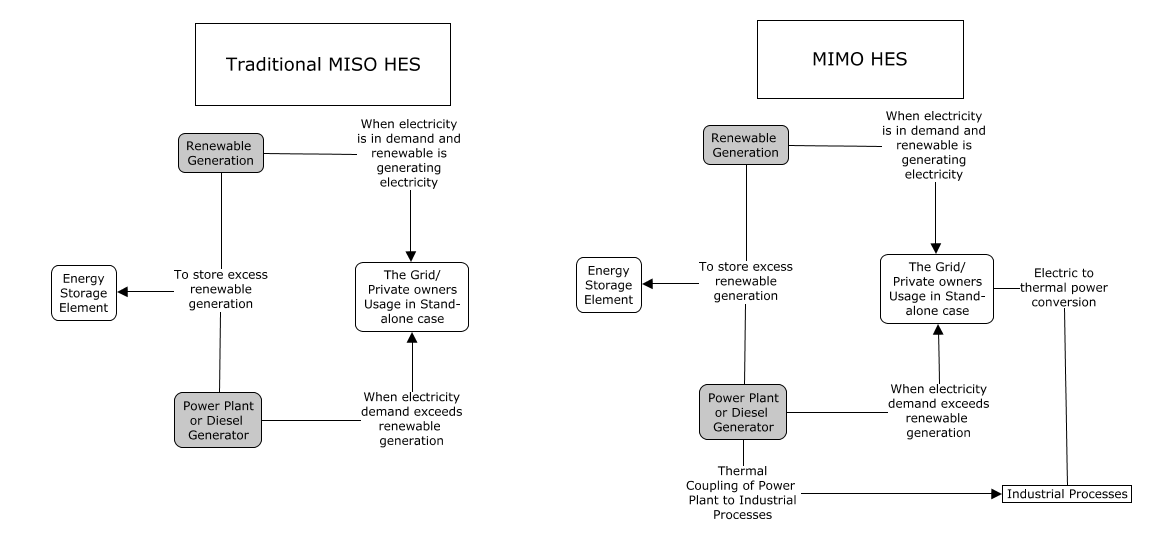
\includegraphics[width=\textwidth]{MISO_MIMO.png}
\caption{\small \sl This figure compares the MISO and MIMO configurations, demonstrating the differences between traditional hybrid energy systems that are focused on generating reliable electricity and non-traditional hybrid energy systems, which have the added objective of generating an additional product.  While many of the elements are the same, the MIMO system includes an Industrial Process  that is either thermally or electrically coupled.}
\end{figure*}

\section{Nuclear Renewable Hybrid Energy Systems}
Nuclear Renewable Hybrid Energy Systems (NRHES) are defined by Bragg-Sitton et al. (2014) as the "tighter coupling of nuclear and renewable energy sources in a manner that better optimizes energy use for the combined electricity, industrial manufacturing, and transportation sectors capable of apportioning thermal electrical energy to first meet the grid demand (with appropriate power conversion systems), then utilizing excess thermal and, in some cases, electrical energy to drive a process that results in an additional product \cite {Bragg-Sitton2014}".  The benefits to the participants of the NRHES that co-locate their facilities include minimizing systemwide costs to the NRHES while increasing economic resilience by diversifying both the means of generating energy as well as the products produced. For example, if natural gas prices increase, the NRHES could rely less on the natural gas plant and put more focus on storage.  If short-term electricity prices are negative, the energy produced by the NRHES can be diverted to the industrial process.

The additional industrial products include, but are not limited to: synthetic fuel, titanium, desalinated water, hydrogen, aluminum, and heat pumps \cite{Bienvenue2015}. The NPP diverts the energy it generates between the grid and the industrial process to maximize profit. The system can allocate energy based on the market value of each of the multiple outputs produced. In the case of a NPP coupled with a desalination plant, for example, if the price of electricity is low, more thermal and/or electric energy can be diverted to generate more clean water at a higher profit \cite {Chen2016}. The costs of running a dynamic system, such as the case with a NRHES, include additional wear and tear, decreased thermal efficiency  due to variability, and increased complexity of operations  \cite{Garcia2013}. The total net costs of the system, such as meeting regulatory expectations , have yet to be determined.

\section{Ongoing Modeling Research}
There have been no physical demonstrations to date of NRHES. Therefore, research has largely focused on computational modeling to determine the feasibility and optimization of coupling elements \cite{Rabiti2015, Boardman2013, Shropshire2012}. Our literature review revealed that much of the work on NRHES is in the design and analysis stage \cite{Epiney2016, Boardman2013, Shropshire2012}. Research has focused on developing models that can dynamically simulate the contributions of variable energy sources, the constraints of fluctuating electricity demand, and thermal/electrical power demands for various industrial processes. The models focus on answering questions regarding minimizing the cost of electricity and ensuring profitability for each of the components comprising the NRHES. In order to move forward with development of any NRHES, such systems must demonstrate that they can be profitable and can reliably respond to fluctuating electricity production and demand \cite{Rabiti2015}.

An ongoing effort at Idaho National Laboratory (INL), Argonne National Laboratory (ANL), and Oak Ridge National Laboratory (ORNL) focuses on modeling a generic NRHES to optimize the size of the components as well as the overall functioning of the system. The generic nature of the plant means that regional variability in the renewable energy produced as well as the costs of the feedstocks for each of the systems is not taken into consideration. The generic model will test the economic viability of NRHES to determine if future development should be pursued. The industrial plant combines a nuclear power plant, a wind farm, a natural gas power plant, a battery, and a high temperature steam electrolysis hydrogen production facility. More component models will be developed in the future that can compare various industrial customers\cite{Harrison2016}. The chosen renewable source, a wind farm, models a highly stochastic system due to the unpredictable nature of wind generation \cite{Chen2016_wind}. The model optimizes the sizes of the nuclear power plant, the natural gas plant, and the battery. The model performs two optimizations, the first on the size of the components and the second optimizing the functioning of the system to minimize costs \cite{redfoot_rabiti_2018}. The objective is to choose the NRHES configuration that minimizes costs while meeting set emissions and grid reliability expectations.
\section{Computational Tools}
NRHES sit in an interesting location in computational modeling. There are many tools to model and optimize non-nuclear hybrid energy systems (HOMER, Hybrid2, SOLSIM, SOMES, ARES, RAPSIM, HOGA) \cite {Bernal-Agustin2009}. These programs generate mass flow and calculate electricity output and the possible output of another product, such as hydrogen. Modelica and Excel, while neither specifically HES nor NRHES tools, have been used to model both nuclear and non-nuclear hybrid energy systems \cite{Shropshire2012, Chen2016, Binder2014, Garcia2015, Epiney2016}. HES tools are typically bought (or developed?) for microgrid standalone systems. The main challenges to applying HES systems to a NRHES are the scale of the system being modeled and fluctuating grid demand.
\section{NRHES Models}
Selecting a tool to model a NRHES requires understanding what characteristics a model must possess in order to provide accurate information. For example, as discussed below, it is important for a NRHES model to incorporate the dynamic nature of the system in order to include losses from the fluctuations in the system. Understanding the differences among the underlying mathematical models as well as the software functionality is essential in determining whether and how a nuclear fuel cycle simulator (NFCS) will be useful to NRHES modeling.
As mentioned above, the model currently under development by Oak Ridge National Laboratory, Argonne National Laboratory, and Idaho National Laboratory has reviewed the essential characteristics for a computational model of NRHES. Rabiti et al. (2015) discusses the important elements of a NRHES computational model in detail, describing the basic requirements of the software as a "computational representation of the thermal, mechanical, chemical, and electrical processes in the systems as process units, reactors, manufacturing plants, and energy delivery (to the appropriate point of interface with the market transaction, such as an electricity bus, or a product depot or distribution terminal where a commodity price is established)"\cite{Rabiti2015}. The model in development by the national laboratories combines RAVEN (Reactor Analysis and Virtual Control Environment) for the stochastic and statistical aspects of the system, such as generating synthetic wind data and optimizing the systems with Modelica for modeling the various components in the NRHES.
\section{RAVEN}
The RAVEN tool was initially built for probabilistic risk assessment. As a probabilistic tool, RAVEN is "able to perform parametric and stochastic analysis based on the response of complex system codes\cite{RabitiRAVEN}." For example, RAVEN can run thousands of different wind energy generation paths to produce a statistically fair representation of how wind power would likely function over any given hour. RAVEN can also generate generic seasonal wind generation over a week. The week long synthetic wind data for summer, winter, and fall/spring can then be extrapolated to represent the whole season, which, in turn, can be extrapolated to represent however long of a time frame is desired to run the NRHES simulation. While the current goal is to create a generic model, it can be tailored to specific regions, defining the costs of inputs such as water and natural gas based on the typical regional price, as well as selling the electricity for the current regional rate. Using synthetic generated data instead of historic data avoids the critique that the model only represents past behavior and is thus inapplicable to future trends \cite{redfoot_epiney_2016}. RAVEN is also used to determine high-risk time series samples to ensure that high risk scenarios are accounted for when desired in a study. In addition, RAVEN can calculate the loss of load probability and the sensitivity to uncertainty analysis due to the figures of merit reliance on a probabilistic approach.

\section{Dynamic Modeling}
Garcia et. al. (2013) and Du et. al. (2014) apply dynamic approaches to modeling hybrid energy systems (HES) to appropriately address the impacts of flexible operation of the system due to variable renewable generation \cite{Garcia2013, Du2014}. In Du et. al. (2014). Two optimization problems are addressed: the first minimizes variability in the HES through optimizing components of the HES system, and the second imposes operating and capital costs on the design variables. Garcia et. al. (2013) has a two-part series. The first applies and analyzes performance of a dynamic approach to modeling some of the physical components of a traditional and an advanced (which produces goods besides electricity) HES. The second paper focuses on economic effects using a dynamic approach, as opposed to time series or statistical analysis. Overall, both parts of the series focus on how a dynamic approach better models the high level of variability of a HES for output generation and profitability maximization \cite{Garcia2013}.
The costs of operating in a flexible manner, dynamically allocating resources between multiple coupled systems, are substantial enough to require a simulation that models the variability of the system at a high fidelity \cite{Garcia2013, Shropshire2011, Locatelli2015}. The dynamic modeling at this point focuses on the dynamic transfer of energy to different sources, and how this transfer impacts the economics and grid reliability. The dynamic allocation of the heat and electricity depending on the renewable generation and the grid demand is an essential characteristic of an NRHES.  Including factors such as how quickly the NRHES will be able to switch between providing energy to the industrial facility and the grid will impact determining whether a NRHES is worth pursuing.  To account for the dynamic nature of the system, NRHES requires either a continuous dynamic model or a high fidelity discrete  model with a very short time step, in the range of an hour at worst, and preferably in the minute scale.
\section{Modelica}
Modelica is a widely used open source language for modeling large and complex systems composed of smaller component models. It is particularly optimized for modeling dynamic systems, making it an attractive language for an NRHES. Modelica has powerful libraries, such as Thermopower, that include the thermalhydraulic modeling tools required for modeling mass flows in energy systems \cite{Binder2014}. The language is well-maintained, giving it the added benefits of having up-to-date documentation and a community that can provide support. Typically, Modelica is run on the Dymola developer environment, a private tool developed by the creator of Modelica, Dr. Hilding Elmquist. Another option for running the Modelica language is the open source OpenModelica environment.

The Modelica HES model developed in Binder et. al. (2014) includes a nuclear reactor, two steam cycles, a chemical plant, and an electrical component \cite{Binder2014}. The products of this Modelica NRHES model are synthetic fuel and electricity. The model includes the ramp up stage when the reactor initially starts or increases from a lower load. The steam generator connected to the NPP determines which of its turbines to use depending on electricity demand, the 60\% turbine, the 30\% turbine, or the 15\% turbine, which can be used in unison if there is a high demand for electricity. A pressure relief valve releases excess energy unused by the turbines. The wind generation is modeled using the Western Wind dataset from the National Renewable Energy Laboratory (NREL) for an unspecified region in Idaho. Each component in the model was tested individually before being combined. Using the individual component models, verifications were made for the system as a whole. The startup transient state of the model took much greater computation time due to the complex interrelations of the components. Generally, to run a model of a NRHES, including using Modelica, requires a control algorithm, a differential equation that controls how the dynamic system allocates heat. The profitability control algorithm can be adjusted to incorporate varying parameters such as the price of electricity or the cost of natural gas. The study concluded that Modelica is an effective tool for dynamically modeling a HES due to its ability to evaluate control algorithms.

\section{Small Modular Reactors}
For completeness, the use of small modular reactors both as tools for load following and as sources of process heat must be addressed. SMRs are generally defined as nuclear reactors under 300 MWe. SMR designs, such as the one in development by NuScale, combine multiple small reactor modules. Multiple SMRs in combination are a promising possibility for NRHES.  With multiple reactors, individual modules can be assigned to meet the industrial process energy demand, with others solely used for electricity generation. Furthermore, as electricity demand grows, additional modules can be added to the industrial park. Multiple SMRs have a clear means of load following, simply by shutting down those reactors whose energy output is not required due to seasonal shifts and other demand factors. The modularity of the SMRs allows greater flexibility in the design of the industrial park.  Locatelli (2015) discusses the technical and economic feasibility of load following using multiple small modular reactors (SMRs), applying the excess energy toward generating algae-biofuel and desalinated water \cite{Locatelli2015}. He discusses the benefits as well as drawbacks of an NRHES that includes a thermal desalination process. A desalination plant has the benefits of switching between a latent and producing state and generating a product that is readily stored. The main drawback is poor water quality and output level when the desalination unit restarts.
\subsection{Other Research on NRHES Models}
Many more studies on HES and NRHES incorporate economic and technical modeling, but the essential characteristics of ability to model a dynamic and stochastic system have been covered. Some other relevant studies include:
\begin{itemize}
\item Shropshire et. al. (2012) does not focus on HES, but discusses how different models of flexible and small modular reactors could integrate into the European energy market with growing renewable generation, thus fulfilling the growing need for flexibility and load following in other electricity suppliers \cite{Shropshire2012}.
\item Shropshire et. al. (2011) develops target cost estimates for reactors given certain economic environments based on competing technology energy costs \cite{Shropshire2011}.
\item NEA-OECD (2011) presents an overview of the capability of implemented newer and older nuclear power plants to load follow \cite{Nuclear2011}.
\item Baker (2016) analyzes the levelized cost of electricity (LCOE) as the figure-of-merit (FOM) and the role of battery storage to evaluate different NRHES scenarios \cite{Baker2016}
\item Kazimi et al. (2009) produces a preliminary dynamic analysis of two NRHES systems that have high levels of renewable energy generation and multiple outputs from the system. The study concludes that NRHES could lead to optimized energy use, reduced carbon, favorable economic performance, and flexible operation time \cite{Kazimi}.
\item Forsberg et. al. (2009) discusses using nuclear power to create more liquid transportation fuels from biomass and fossil fuel sources \cite{Forsberg2009}.
\item There have also been two regional modeling studies done on Texas and Arizona focused on including regional characteristics to determine the renewable used and the industrial process.
\end{itemize}
Table I displays the characteristics routinely described as necessary to model a NRHES along with their citations.

\begin{table}[h!]
\centering
\caption{References for Each NRHES Characteristic}
\begin{tabular}{ ||c | c|| }
 \hline
 NHES Characteristic & Paper \\ [0.5ex]
 \hline \hline
 Dynamic & \cite{Garcia2013, Du2014, Kazimi, Garcia2016}\\
 \hline
 Sensitivity Analysis & \cite{Shropshire2011, Rehman2010, Adaramola2014, Chen2016}\\
 \hline
 Optimization of components & \cite{Chen2016,Ozcan2016, Forsberg2009,Garcia2015,Aumeier2011}\\
 \hline
 Stochastic Model of Renewables & \cite{Rabiti2015, Garcia2016,Locatelli2015}\\
 \hline
 Grid Demand model & \cite{Forsberg2013, Garcia2016,Garcia2013,Ruth2014,Chen2016}\\
 \hline
  Economic FOMs & \cite{Garcia2016,Chen2016,Rabiti2015,Epiney2016,Bragg-Sitton2014}\\
 \hline
\end{tabular}
\label{table:1}
\end{table}

The table displays the characteristics that arise as a pattern in many of the documents.  The six characteristics included in the table are those likely necessary for a NRHES model.  Each of the characteristics has been included in previous studies, and thus has some already proposed approaches.  The characteristics can be studied in greater detail in order to determine if they satisfactorily model the system. A NFCS would need to find a way to appropriately include these characteristics.
\section{Nuclear Fuel Cycle Simulators}
The common uranium nuclear fuel cycle describes the system of mining uranium, converting the uranium to gaseous $UF_6,$ enriching the uranium with higher percentages of U235, fabricating the fuel, the fuel changing in the reactor, storing, reprocessing, and final disposal. There are different fuel cycles, depending on the type of fuel used, the reactors included, and how the spent fuel is managed. Nuclear fuel cycle simulators model the fuel cycle determining the likely quantity and characteristics of nuclear fuel in order to determine future policies surrounding management of the spent fuel.
This section identifies basic properties of nuclear fuel cycle simulators and assesses their distinct functionality. Figures 2a and 2b display many of the currently used nuclear fuel cycle simulators (NFCS). The fuel cycle simulators are the central nodes in these figures, with the tools for computing some of the basic descriptive qualities of a fuel cycle branching off. The computational attributes that are often included in NFCS are: mass flows, reactor physics, thermal hydraulics, reprocessing, waste management, risk management, and economics. While different fuel cycle simulators were initially optimized for a variety of applications, there is a lot of overlap in their functionality \cite {Guerin2009}. Because nuclear fuel cycle simulators are attempting to model the same thing, the nuclear fuel cycle, the models include some means of tracking the isotopic makeup of the fuels as they move through the fuel cycle. The different fuel cycle simulators generally have the ability to simulate fleets of nuclear reactors with the associated fuel cycle industrial processes and nuclear materials storage. As can be seen in figures 2a and 2b, there are a good number of NFCS, which all have different functionality and dependencies.
%\begin{subfigures}
\begin{figure*}
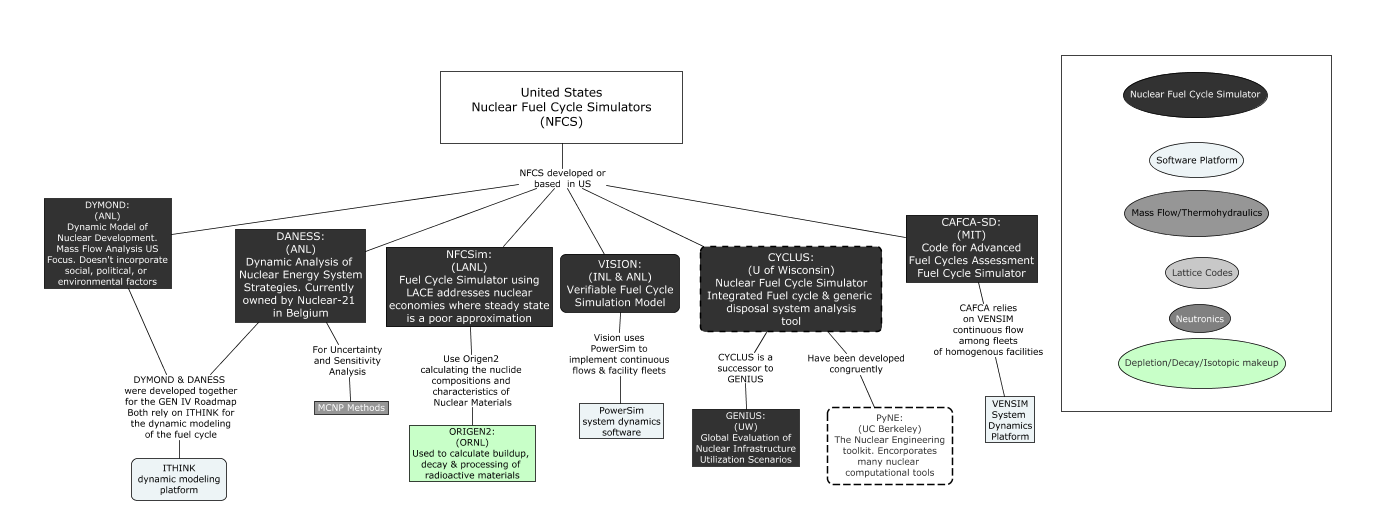
\includegraphics[width=\textwidth]{US_FUEL_TOOLS.png}
\caption{\small \sl This figure displays the nuclear fuel cycle simulators developed in the United States, though they are not necessarily specifically built to demonstrate the development of a US fuel cycle. This figure does not include all nuclear fuel cycle simulators or their dependencies.  The figure demonstrates some of the complexity of current Nuclear Fuel Cycle Simulator options. The figure demonstrates the types of tools NFCSs depend on, thereby suggesting some of their functionality.}
\end{figure*}

\begin{figure*}
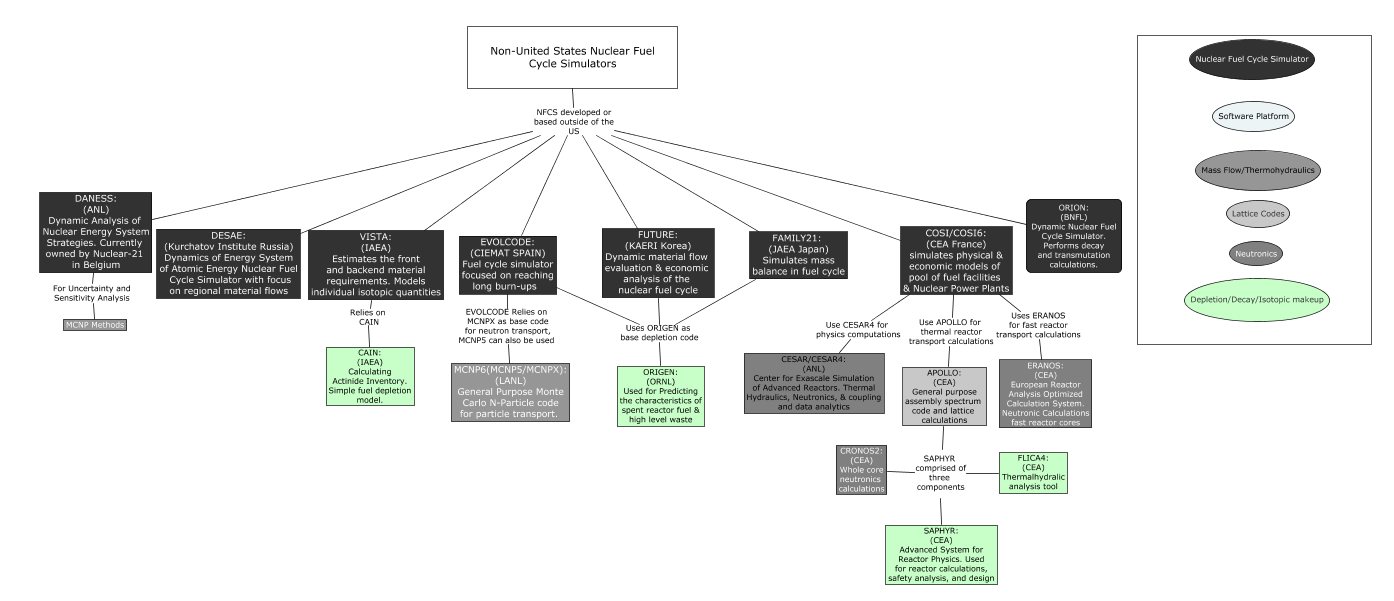
\includegraphics[width=\textwidth]{Non-US_FUEL_TOOLS.png}
\caption{\small \sl This figure displays the nuclear fuel cycle simulators developed outside of the United States. The full relationship between the various computational tools may not be covered.}
\end{figure*}
%\end{subfigures}
In the case of the once-through fuel cycle, uranium is mined, enriched for a higher concentration of U-235, molded into fuel assemblies, and used in a nuclear reactor for between 36 and 72 months. The spent fuel is not reprocessed, so it is first stored on site in spent fuel pools, then canisters. Eventually, the spent fuel will be deposited in a deep geologic repository. More advanced fuel cycles involve different degrees and methods of used fuel reprocessing. Nuclear fuel cycle simulators permit modeling of new techniques applied to all parts of the nuclear fuel cycle; from the mining through the waste management. The idea behind modeling the full nuclear fuel cycle is to optimize the fuel cycle given technical, environmental, regulatory, and economic constraints.

Prof. Paul P. H. Wilson reported for the Blue Ribbon Commission on America's Nuclear Future "Comparing Nuclear Fuel Cycle Options" discusses, at a high level, different nuclear fuel cycle simulators' performance for a once-through system, a limited recycling option, as well as continuous recycling. Prof. Wilson describes nuclear fuel cycle simulators as focusing "on understanding mass flows and facility deployments under alternative civilian nuclear fuel cycles, particularly during transitions between fuel cycles." The two uses for a NFCS as stated in the report are to make informed policy decisions and to determine more fine-grained technical decisions about what technologies to pursue. Prof. Wilson breaks down some of the assumptions either explicitly or implicitly included in the nuclear fuel cycle simulators, including:
\begin{itemize}
\item "Growth rate of nuclear electricity,
\item Date of introduction of new technologies and facilities,
\item Constraints on spent fuel interim storage capacity,
\item Constraints on spent fuel storage/cooling times,
\item Constraints on quantity of separated plutonium,
\item Relative priority of different fuel cycle paths, and
\item Supply vs. demand flow control at each fuel cycle stage."
\end{itemize}

Prof. Wilson explains that a degree of uncertainty present in each of the assumptions introduces even greater variability. NFCS differ both in how they calculate their FOMs as well as in how the FOMs are presented. Benchmarks for NFCSs often entail summaries for each fuel cycle simulator by the authors of the tool \cite{Guerin2009}. Making comparisons of various tools is difficult because most of the tools are proprietary. As a result, the reports of the developers are the main access to understanding the tool rather than using a controlled end user. Different authors choose to discuss different aspects of the NFCS, adding to the difficulty of comparing the various NFCS. Even when two NFCSs have similar functionality, it can be hard to make comparisons based on benchmark reports due to different emphases in the reports describing the tools. This variability leads to model development with built-in biases that weigh certain characteristics of a technology as more important, thereby skewing the results.

Due to the uncertainties, NFCSs are best used as comparative tools, as opposed to predicting absolute values \cite{Wilson2012}. Given different constraints within an NFCS, it can demonstrate the relative differences between the two simulations better than the absolute nature of either one. The strength of relative comparisons is especially clear in economic analyses, where prices and how they are likely to change over time are unpredictable. The simulator, if built well, would be able to show which model would be cheaper, but not exact prices\cite{Wilson2012}. Some of the uncertainty concerns surrounding simulating a nuclear fuel cycle as stated by Prof. Wilson:

\begin{itemize}
\item Cost of water
\item Uranium consumption and costs
\item Total land use
\item Waste disposal space
\item Localized variations of the estimated peak dose rate
\item Radiotoxicity of waste streams
\item Radioactive liquid and gaseous release volumes
\item Conventional pollutant release over the lifecycle of the nuclear system
\item Required Enrichment of the fuel
\item Attractiveness of separated materials for proliferation of nuclear weapons
\item Difficulties in siting a nuclear power plant, and
\item Variation in how metrics are calculated.
\end{itemize}

Many of the above listed characteristics are region-specific capital, operations, and maintenance costs that would also apply to NRHES.  In order to include these characteristics for both the nuclear fuel cycle and NRHES, some measures of uncertainty would need to account for the variability of circumstances. Wilson breaks down the uncertainties into the categories of cost, safety, resource utilization, sustainability, and non-proliferation ~\cite {Wilson2012}.

The major difference between many of these nuclear fuel cycle simulators is the ability to model discrete facilities and fuel batches versus modeling continuous mass flows throughout the fleet of facilities operating in an identical fashion. In the case of the fleet modeling, the average value for each of the facilities is assumed. The discrete model requires more information, such as the fuel composition for each type of reactor included in the simulation, while providing a more detailed analysis. As a result, the discrete model is more computationally complex and expensive.

In "Modeling the Nuclear Fuel Cycle," Juchau et al. (2010) describe four functions as necessary for a NFCS to meet the desired qualities of a proposed organization called the Simulation Institute for Nuclear Enterprise Modeling and Analysis \cite{Juchau2010}. The four functions, which reiterate the characteristics described by Prof. Wilson, include:

\begin{itemize}
\item "Characterize and deploy individual fuel cycle facilities and reactors in a simulation while discretely tracking material movements,
\item The capability to perform an uncertainty analysis for each element of the fuel cycle and an aggregate uncertainty analysis,
\item Inclusion of an optimization engine able to optimize simultaneously across multiple objective functions, and
\item Open and accessible code software and documentation to aid in collaboration between multiple entities and to facilitate software updates."
\end{itemize}

Juchau (2010) reviews the nuclear fuel cycle simulator tools CAFCA, COSI, CEPMNFC, DANESS, NFCSim, VEGAS, VISION, NFCSS, and GENIUS 1. His conclusion is that many of these tools have overlapping functionalities, partly due to the proprietary nature of at least components of each. One reason why there are so many nuclear fuel cycle simulators is that many of the countries that currently have NPPs have designed their own simulators. Figure 3 depicts the non-US NFCSs along with some of their software dependencies. Most of the fuel cycle simulators are not open source or available for download; thus, each nation tends to have proprietary software. As discussed with Prof. Kathryn D. Huff, it is also often more efficient, both in terms of time spent as well as better integration, if the different functions are designed by the same team \cite{redfoot_huff_2016}. Integrating components, such as a burnup calculation, from one system into a new system can often be more challenging than building the function from scratch. While sharing code can be challenging among various programs, some calculations or libraries are commonly used by NFCSs. For example, Figure 3 depicts EVOLCODE, FUTURE, and FAMILY21 as all relying on Origen.
\chapter{Methodology of Modeling a NRHES with a NFCS}
The underlying structure of passing materials between various facilities is similar enough between nuclear materials in a fuel cycle and heat or electricity flow in a nuclear hybrid energy system that a nuclear fuel cycle simulator could theoretically model a nuclear renewable hybrid energy system. In the case of a NRHES model, the facilities are the NPP, the renewable, and the industrial process at least.  In the case of the nuclear fuel cycle, the facilities are the steps in the given fuel cycle. Both systems are time dependent and include uncertainty measures. Many of the uncertainty measures found in NFCS are the same for NRHES including O\&M costs, water costs, and challenges in siting a nuclear power plant. The uncertainties can be accounted for using sensitivity analyses. Optimally, both systems would be:
\begin{itemize}

\item flexible so that new component models and specific regional characteristics could easily be added,
\item open source so that researchers can use the tools instead of rebuilding already available tools, and
\item usable by technical and non technical people alike to address policy decisions.
\end{itemize}

A NFCS must be able to reasonably model the dynamic nature of NRHES. The dynamic aspects of concern are how the energy would switch between different loads as well as the ramping of various generation components.  The length of the simulations and time step are vastly different between NRHES and the fuel cycle. The nuclear fuel cycle does not require the quantities to be exchanged nearly as regularly as a nuclear hybrid energy system and with as inconsistent of quantities. While the fuel cycle may be run with a monthly time step and the same resource amount is exchanged at each time step, a NRHES requires a variable amount of resource to be exchanged on an hourly or minute-to-minute scale. The dynamic impacts on the physical system must be included in order to generate a meaningful model of a NRHES. The stochastic aspect of the renewables components of a NRHES also requires either external coupling with a tool able to model randomness such as RAVEN or the use of real time data from a specific region. The dynamic and stochastic components of modeling a nuclear hybrid energy system require some work to incorporate.

Many of the features commonly found in a NFCS would not be needed in a NRHES model.  There would be no need to model a fleet of NRHES at this point in development, so a system would have to be able to model discreet facilities.  The reactor calculations, such as burnup, would not be needed for a NRHES.  The back end of the fuel cycle, such as models for reprocessing and long term waste storage would also not be applicable at this point to a NRHES model.  The primary qualities that would be used are optimization methods, economic evaluation, and means of exchanging materials in a system.

The nuclear fuel cycle shares similar enough underlying characteristics with a nuclear hybrid energy system to loosely model the system.  A more thorough analysis of the benefits and challenges to using a NFCS to model NRHES will be discussed surrounding the model. A NFCS that is in a mature state of development, open source, easy to incorporate new components, flexible enough to change the materials exchanged rapidly, and able to be coupled with external tools for modeling the renewable resource could speed up the development of a NRHES model. Cyclus is the only currently open source nuclear fuel cycle simulator.  As such, Cyclus has distinct advantages among the NFCSs when developing an NRHES.

\section{Cyclus}

The flexibility and modular design of Cyclus suggest its potential to successfully model a NRHES. The Cyclus fuel cycle simulator's underlying system is the dynamic resource exchange (DRE) \cite{Huff2016}.  The DRE has a set time step at which point certain facilities will put their resources on the market for exchange while other facilities can make a bid for the desired amount of the resource. For example, in the case of modeling the nuclear fuel cycle, the reactor could declare how much spent fuel it has once every eighteen months.  A reprocessing facility and a long-term geologic repository could both bid on how much of the spent fuel each facility could take at that point.  The DRE has a built in functionality of preferences for allocating a resource.  For the example given, a preference could be a built in for the reprocessing facility, meeting the bid from this facility before sending the remaining spent fuel resource to the long-term geologic repository. The simulation could be run over hundreds of years to demonstrate the accumulation of spent fuel and fission products over the entire timeline.

The NRHES model built in Cyclus will determine whether the DRE is sufficiently flexible to model other systems besides the nuclear fuel cycle.  In the case of a NRHES, the DRE would be passing the electricity or heat to the various facilities.  For example, the reactor could  pass heat to the industrial process at a time step of one hour or one minute and send electricity to the grid.  The renewable would pass electricity to the grid when generating.  The grid would make a bid every time step for how much electricity is demanded.  The industrial process would also make a bid for the heat and/or electricity required.  The built in preferences functionality in Cyclus could be used to ensure the resource is sent to the facility willing to pay the highest price for the resource.  Thus, the electricity or heat could be sent to the industrial process when the product created with that energy is worth more than the current value of electricity on the grid.
\chapter{Thermal Versus Electrical Coupling}
From the literature review on NRHES, a notable gap in the current research is modeling the benefits gained from thermally coupling systems as compared to electrically coupling.  The efficiency benefits would have to be greater than the costs associated with co-location.  Cyclus's ability to dispatch resources could allow for a comparison between coupling an industrial process thermally or electrically. The Cyclus model developed for this research will be used to compare a system that exclusively produces electricity, but varies in the amount of electricity sent to the industrial process, with a system which sends process heat directly from the reactor to the industrial process as well as sending electricity to the grid.

\chapter{Figures of Merit}
To determine the performance of an electrically coupled versus a thermally coupled NRHES with the Cyclus model, clear performance criteria must be established.  While economic figures of merit must be evaluated for a NRHES, other benefits of the system such as grid reliability and safety of the system should also be considered. This section of the thesis details the current efforts at establishing a figure of merit to analyze a NRHES and suggests two approaches to future assessment, Analytic Hierarchy Process (AHP) and a dimensional analysis approach.
\section{Economic Figures of Merit}
\subsection{Levelized Cost of Electricity}
The levelized cost of electricity (LCOE) is the typical FOM for comparing the profitability of different generating sources, such as nuclear, fossil fuels, and renewables. The LCOE is mathematically defined as the costs of a power-generation source divided by the total energy output, with units of \$/unit of energy. The LCOE is easiest to think about as the lowest average amount of money a project can sell the electricity generated for over in order to break even, or for the Net Present Value (discussed below) to equal zero. The LCOE is a ubiquitous metric used for evaluating energy generation sources, but it is not always calculated the same way.  The two equations below illustrate very different means of calculating a figure bearing the same name.  While a lack of clarity about what is meant by LCOE can be mitigated by defining the means of calculating the value, this practice is often overlooked.
Ted Baker, in Analysis of Nuclear Hybrid Energy Systems with Battery Storage Using Levelized Cost of Electricity, evaluated the effectiveness of the levelized cost of electricity (LCOE) for a hybrid system \cite{Baker2016}. His analysis found the LCOE was incapable of fully capturing the benefits of energy storage associated with a NRHES and did not including all revenue streams.  Baker defines the utilization as energy used divided by the total possible generation. In order to normalize the LCOE, the calculated LCOE shown in equation 1 below is multiplied by the total energy actually used for each source.  As Baker describes, to normalize the LCOEs "the sum of all specific LCOEs is then divided by the sum of the demand data. This weights each source by its contribution to coverage (pg. 20)."  The revenue rate of the secondary product in \$/MWh is subtracted from the total LCOE in order to find the net LCOE.  Baker concludes that the LCOE is ineffective for the revenue stream of a secondary product and includes errors for variable generation and battery storage. Baker recommends exploring more advanced LCOE and Levelized Cost of Storage (LCS) calculations. The LCS focuses on comparing the costs between various energy storage sources optimizing for different use cases \cite{Tyskiewiczd}.

\subsection{Levelized Avoided Cost of Electricity (LACE)}
The levelized avoided cost of electricity focuses on including fluctuating renewables by determining the money saved by the dispatchable resource for not having to produce that energy. With dispatchable resources whose costs largely come from their fuel source, such as fossil fuels based generation sources, there is a savings for the fossil fuel plant for not having to produce the electricity.  For nuclear power, whose costs come almost entirely from sunk in capital costs, there is very little avoided cost for not producing the electricity generated from the renewable.  LACE applies specifically to renewables and will be interesting to include as a FOM for a NRHES as a fossil fuel, a nuclear, and a renewable generation source are all present. The LACE will be different depending on whether the renewable generation replaces the nuclear or fossil fuel power plant.
\subsection{Net Present Value}
Net Present Value (NPV) is generally considered to be the present value of a system at a given required internal rate of return (IRR) compared to the initial investment. The question a NPV analysis tries to answer is whether, based on the overall profit, a project is worth investing in.  The NPV includes whether the money invested in a project will make more of a profit over its lifetime than simply leaving the money in the bank.  In terms of comparing NRHES with different industrial processes, it is a metric that compares the likely profits received from each.  The net present value determines the LCOE of a project over its lifetime by finding the internal rate of return.  The Internal Rate of Return (IRR) is "the interest rate at which the net present value of all the cash flows from a project or investment equal zero."  The IRR is the interest rate that either the money spent on the NRHES would earn if it is kept in the bank, or the profit over the lifetime NRHES would earn.  The net present value needs to include a grid reliability metric and a value for non-emitting energy to fairly represent a NRHES.
\section{Grid Reliability}
A hybrid energy system in general has not only a goal of profitability, but to ensure a reliable source of energy, especially from a system that includes fluctuating sources of energy. The system would, therefore, benefit from an evaluation of the reliability of the energy generated as well as an economic evaluation.
\subsection{Loss of Load Probability (LOLP)}
The loss of load probability (LOLP), is "a measure of the probability that a system demand will exceed capacity during a given period; often expressed as the estimated number of days over a long period, frequently 10 years or the life of the system" \cite{Electromn}. The LOLP was originally introduced in 1947 by Giuseppe Calabrese and has since become a standard grid reliability metric \cite{calabrese1947generating}. The LOLP can be mathematically shown, as described in Hattab et. al. (2015), as \cite{Hattab2015}:
\begin{equation*}
LOLP =\sum_{j} P_jt_j\,.
\end{equation*}

Where P(j)*t(j) is the contribution that a particular outage of some magnitude O(j) has on the overall risk of a load greater than the reserve. t(j) is the number of days that an outage of some magnitude O(j) would cause a loss of load in the system\cite{Hattab2015}.

One major goal of a NRHES is to minimize the number of days that the system cannot meet the grid demand.  With fossil fuels, nuclear, and renewables all contributing, along with a battery, considerable backup ensures that grid demand is met. For a NRHES, two LOLPs must be generated; one for meeting the electricity demand from the grid and one for meeting the energy needs of the industrial process.  If the industrial process intends to fluctuate its output along with the energy generated from renewable and the grid demand, the losses from the industrial process will need to be taken into consideration for grid reliability. In order to fairly evaluate the benefits of an NRHES, metrics describing the system need to include a grid reliability component.
Eventually, the goal is to determine a figure of merit that is able to incorporate grid reliability and profitability metrics.  The profitability metrics will include the materials replacement rates for different reactor types, industrial processes, and heat transport mechanisms. Future work will include emissions in the FOM. Since at this point, standard figures of merit have not been established for NRHES, this research will work to determine some combination to evaluate the systems.


Here ends what I will send for a review to my committee.

\chapter{Applying Risk Assessment Techniques to NRHES}
Identifying likely failures is an important aspect of safe and secure operation of any large infrastructure. For a NRHES, a large piece of infrastructure that has as of yet to be built, a design that addresses likely failures ensures long term safe, reliable, and profitable operation.   In order to examine the impacts of a nuclear renewable hybrid energy system, this chapter will evaluate the economic, grid reliability, and physical risks of failures in the coupling of a nuclear power plant to an industrial process which functions in a dynamic fashion. The dynamic nature of the heat allocation in a nuclear hybrid energy system results in uncertainties both in the reliability of the energy demanded by the grid as well as that demanded by the industrial process. The focus of this section is to develop a means of comparing various NRHES configurations to determine which NRHES configuration will be used in the Cyclus model.
\section{Risk Assessment Background}
Risk assessment is a means of analyzing complex systems for hazards. Often the risk assessment tools; such as probabilistic risk assessment, fault tree analysis, and failure mode and effects analysis; model many variables in large systems and attempt to contain them into an easy to understand table or number for comparison. Since there has yet to be a physical model of a NRHES built, now is the appropriate time to assess risks in order to incorporate mitigating measures in the design basis. Risk based design has been used for pyroprocessing and hot cell systems (Borrelli, 2016), though focused on proliferation risks. Incorporating risk management in the design of a facility minimizes the costs and dangers associated with the system in the long run.
	When determining an appropriate electricity generation source for a given region it is important to incorporate variables such as economic viability, emissions, flexibility, and reliability. A NRHES is even more difficult to quantify as it supplies both electricity to the grid as well as a secondary product. The goal is to have a more economically robust system that emits less and is both more reliable and more flexible than any electricity generation source currently available.

\section{Preliminary Hazards Analysis}
As was done in Falcone et. al. in establishing a new approach to risk assessment of cogeneration systems, this risk assessment will begin with a preliminary hazards analysis (PHA). The main purpose for a PHA is, as the name suggests, identify hazards and possible implications of the design of a particular system or product.  A PHA is appropriate for the current state of development for a NRHES due to it still being in the design stage. Since a NRHES is currently in a conceptual phase, the goal of this PHA will be to reduce or eliminate potential economic, reliability, and physical safety hazards. Performing a PHA at this early point in the lifecycle of a NRHES will hopefully reduce the resources spent on engineering design and potential construction errors. As stated in Ostrom et. al.  "a PHA should include the following:

\begin{itemize}
\item Establish for purpose of the analysis
\item Boundaries between the system, any system with which it interacts, and the domain;
\item Overall system structure and functionality
\item Identify
\item Detailed list of hazards of the system based on preliminary hazards list report and the requirements;
\item Update hazards list;
\item Accidents to the most practicable extent
\item Events of accident sequience and those that can be discounted;
\item Record in hazards list.
\item Assign Each accident a severity categorization and each accident sequence a predicted qualitative/quantitative probability target.
\item Document Any safety features that are to be implemented during the design and development phase"
\end{itemize}
This analysis will seek to address the above requirements from an economic, grid reliability, and physical safety perspective of a NRHES. Due to lack of expertise in either the economic or possible physical failures of a NRHES, this analysis is not exhaustive but will hopefully address some of the more obvious concerns. The PHA will need to be added upon as research continues and hazards are determined.
	In order to perform a PHA requires classifying the hazard level and frequency associated with each event. The hazard classes for this PHA range from Negligible to Catastrophic. A Class I hazard has negligible negative outcomes, a Class II hazard has marginal effects, a Class III hazard has critical impacts, and a Class IV hazard has catastrophic impacts (Ostrom et. al., 2012).  The frequency of occurrence, since this system has yet to have a physical demonstration, will be qualitative and an intellectual exercise as the values cannot be verified at this point.

\section{Economic PHA}

\section{Grid Reliability PHA}

\section{Physical PHA}

\section{Analytic Hierarchy Process (AHP)}
Analytic hierarchy process (AHP) is a decision analysis method, a means of comparing various options, based on multiple attributes. For this research, the same NRHES with only the industrial process switched out will be compared. As mentioned before, the three industrial processes being compared for this research are desalination, hydrogen production, and synthetic fuel production. The AHP includes comparing each of the potential options on suboptions. In this case the three industrial processes to potentially be included in the NRHES will be compared based off of economics, grid reliability, and physical safety. These subcomponents can be easily analyzed, thus the AHP provides not only insight into which is the best overall choice given the inputs and weights, but also which is the strongest candidate for each of the components. The AHP is especially applicable at this point in the development of the NRHES due to the relative values of physical safety for example for a desalination plant as compared to a synthetic fuel plant can only be based upon expert judgement. The AHP measures the consistency of the values used to compare the different options using a consistency ratio, which needs to be less than .1, or 10\%, in order to be considered consistent.
The focus for the AHP conducted in this research is on the process of comparing different industrial processes for an NRHES, not on the actual values. In order to find the relative values of the value of 1 MWth for a desalination system versus a synthetic fuel system, for example, would require finding the optimal size of each of the industrial processes for the NRHES and the total costs associated with the process.  Baker, 2016  included calculations for sizing a reverse osmosis desalination plant, capital costs, and O\&M costs.  Baker converted the values of selling the desalinated water from \$/kgal to \$/kWh in order to evaluate the value of the electricity used to generate the product. Future work for determining the optimal industrial process will include undergoing a similar process for hydrogen and synthetic fuel production in order to have appropriate values to input into the AHP.  The tables shown below display the relative values for each of the characteristics considered in the AHP. The values are chosen on a scale of one to five, with the industrial process strongly reflecting that characteristic receiving a five and the characteristic relatively less reflecting those characteristics receiving appropriate smaller numbers. As current research on NRHES focuses on the economic feasibility of the system, economics will be the most strongly weighted at 62.5\% with grid reliability weighted at 25\% and safety at 12.5\%.  While the safety of the system is in reality the most important characteristic, as it is the foundation which the economic and grid reliability characteristics rely on, the safety issues are the most easy to mitigate and the most well known. Safety is also included in the economic and grid reliability metrics. The weights associated with each of the characteristics were found through the numbers associated with the relative priorities from Table 9.

\section{AHP Expert Survey Methodology}
The results from the AHP Expert survey will determine which industrial process is modeled in the Cyclus model.
\section{AHP Results}





\chapter{Future Work}
While there are some interesting potential benefits to a NRHES, such as diversifying sources of electricity production, co-locating the facilities have some potential drawbacks.  Integrating exclusively through the grid results in a decoupling of potentially negative feedback effects \cite{Harrison2016}.  A meaningful model would be able to compare a NRHES to the current grid system. The CYCLUS tool could be used to model the difference between co-locating the given facilities in a NRHES as compared to each of the facilities acting independently at different nodes on the grid.  The DRE could track the profitability of each of the facilities independently, each of the generation sources selling electricity to the grid and the industrial facility producing a product.  The DRE could also treat the system as a single facility that outputs two products, the industrial good and electricity to the grid. Along with profitability, other important figures of merit, such as emissions and hours not meeting the grid demand could be tracked and compared in CYCLUS.

Future research will focus on using CYCLUS as a deployment tool for electricity \cite{redfoot_rabiti_2017}. The DRE would be able to put some quantity of heat or electricity on the resource exchange market.  The industrial process or grid could each bid for the heat using economics or other preference model.  The time step for the DRE would be very short, on the order of a minute, in order for the model to output valuable information.
 New archetypes for the waste heat could also be included in order to determine if uses for waste heat are worth pursuing.  Future research will focus on building the archetypes for allocating the heat and electricity in a NRHES.
\section{Summary Remarks}


\section{Examples of acronyms}
Example of acronym: \ac{cogs}
Using it again: \ac{cogs}
Plural one: \acp{vm}

% --------------------------------------------------------------------------
% --  --


% --------------------------------------------------------------------------
% -- Summary and Conclusions --
\chapter{Summary and Conclusions}
\label{Chapter:SummaryAndConclusions}

Example summary and conclusions. You can refer to chapters and sections using their label, e.g Chapter \ref{Chapter:Introduction}.

% --------------------------------------------------------------------------
% -- References --

\clearpage
\renewcommand\bibname{References} % Relabels bibliography title as "REFERENCES"
\addcontentsline{toc}{chapter}{\textsc{\bibname}} % Adds to table of contents
\bibliographystyle{plain}  % Sets style, plain is fine for this
\bibliography{example-bib-file.bib}  % Name of bibliography file containing your references. It is best practice to have a separate file, as it makes it easier to share your references, make derivative works, or use the references from a prior work (e.g a prior paper that your thesis work is building on).

% Examples of citing GitHub repositories:
%   http://academia.stackexchange.com/a/14015
%   https://github.com/blog/1840-improving-github-for-science
%   https://guides.github.com/activities/citable-code/
%   https://github.com/GhostofGoes/uidaho-masters-thesis/
%   Wait, that last one is recursive...oh no. RIP poorly programmed web crawling spider.




% --------------------------------------------------------------------------
% -- Appendices --
\clearpage
\appendix  % Marks start of appendices

% Appendices are done as LaTeX chapters
\chapter{Your fist appendix}
First appendix content

% ** This is an example of a YAML file listing, but it could be anythig, e.g full experiment results, or list of equipment used. **
% \clearpage
% \chapter{Exercise Specification}
% \lstinputlisting[firstline=56, firstnumber=1, language=yaml,caption=Exercise Specification]{Specifications/exercise-specification.yaml}

% ** Example of a Python script code listing **
% \clearpage
% \chapter{vsphere-info Script Source Code}
% \lstinputlisting[firstline=16, firstnumber=1, language=python, caption=vsphere-info script]{Code/scripts/vsphere_info.py}



\end{document}

% ** DO NOT PUT ANYTHING AFTER THE END OF THE DOCUMENT! **
